% ============================================================================
% ŠABLONY LATEX PRO GRAFY Q1, Q2, Q3, Q4, Q5, Q6
% ============================================================================

% V sekci "6.2 Q1: ROLLUP Dekáda-Rok-Model":
   // po SQL kódu a výsledcích analýzy
\begin{figure}[H]
    \centering
    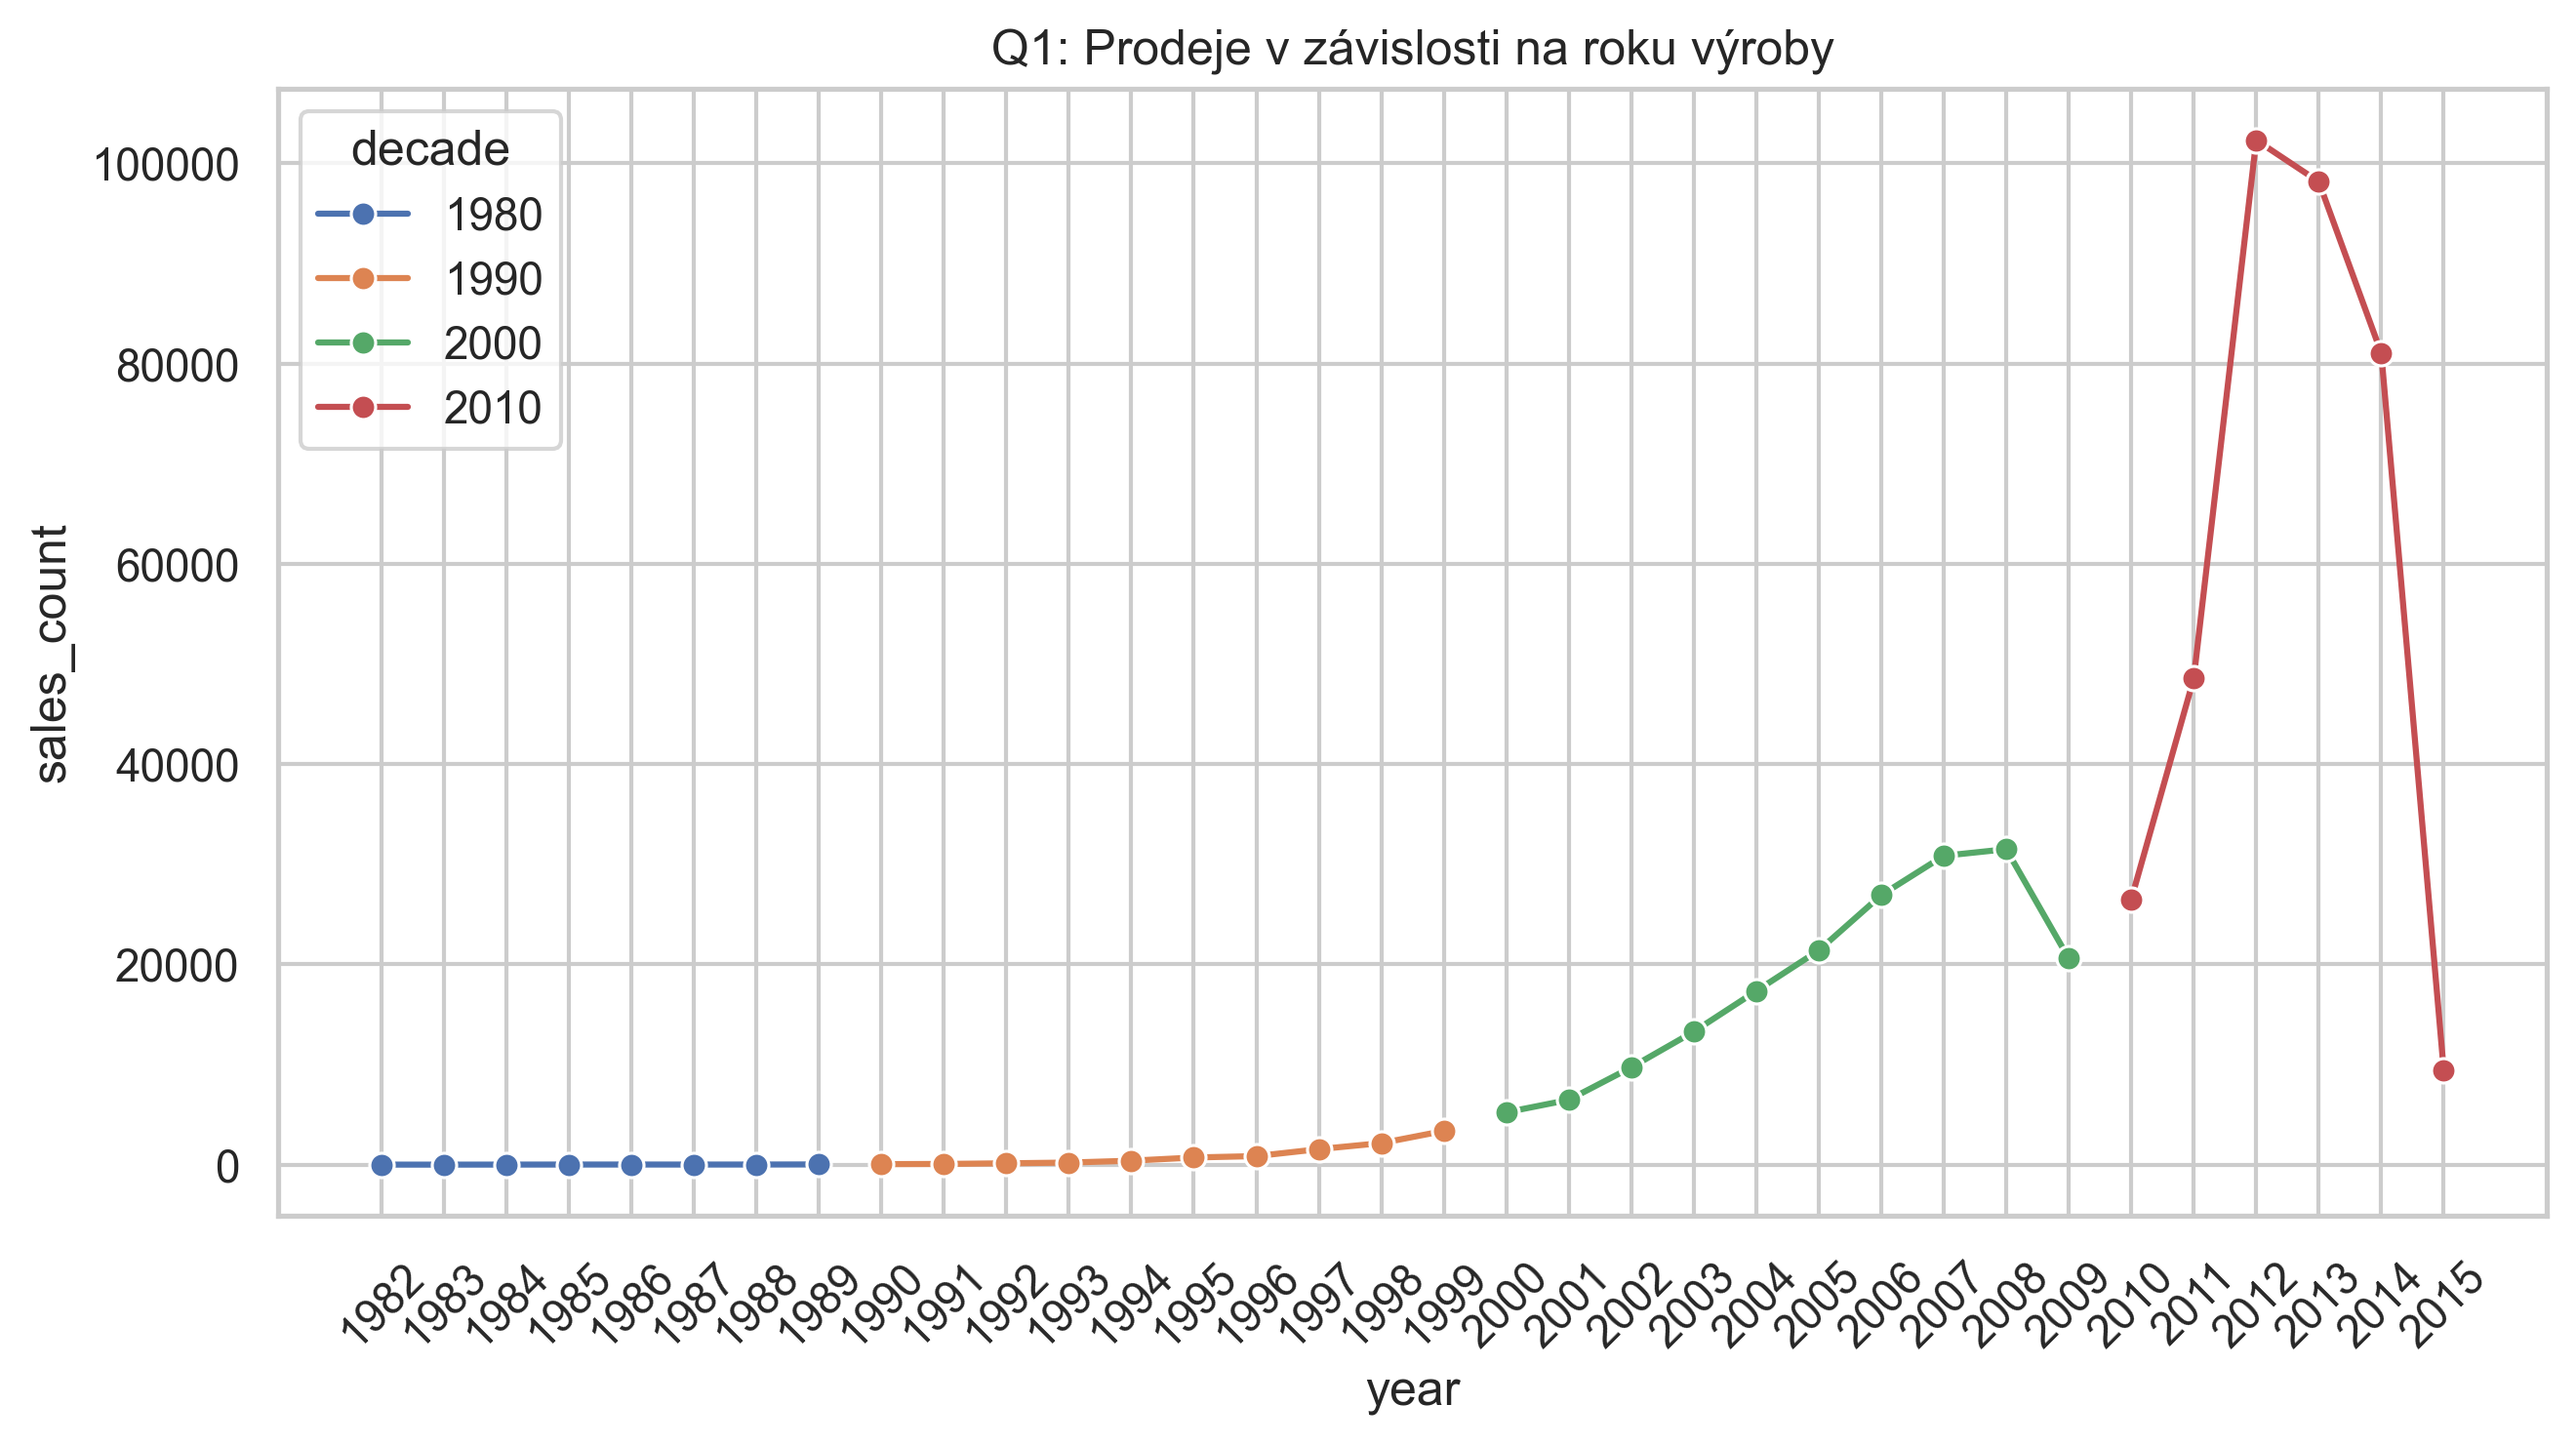
\includegraphics[width=0.85\textwidth]{../output/q1_trend.png}
    \caption{Q1 (ROLLUP): Lineplot prodejů v závislosti na roce výroby – hierarchické mezisoučty dekád. Filtrace na úroveň rok (model NULL) odstraňuje datový šum. Hue (barva) reprezentuje jednotlivé dekády (1990s, 2000s, 2010s).}
\end{figure}

% V sekci "6.3 Q2: CUBE Model-Body-Transmission":
   // po vysvětlení 3D datakrychle
\begin{figure}[H]
    \centering
    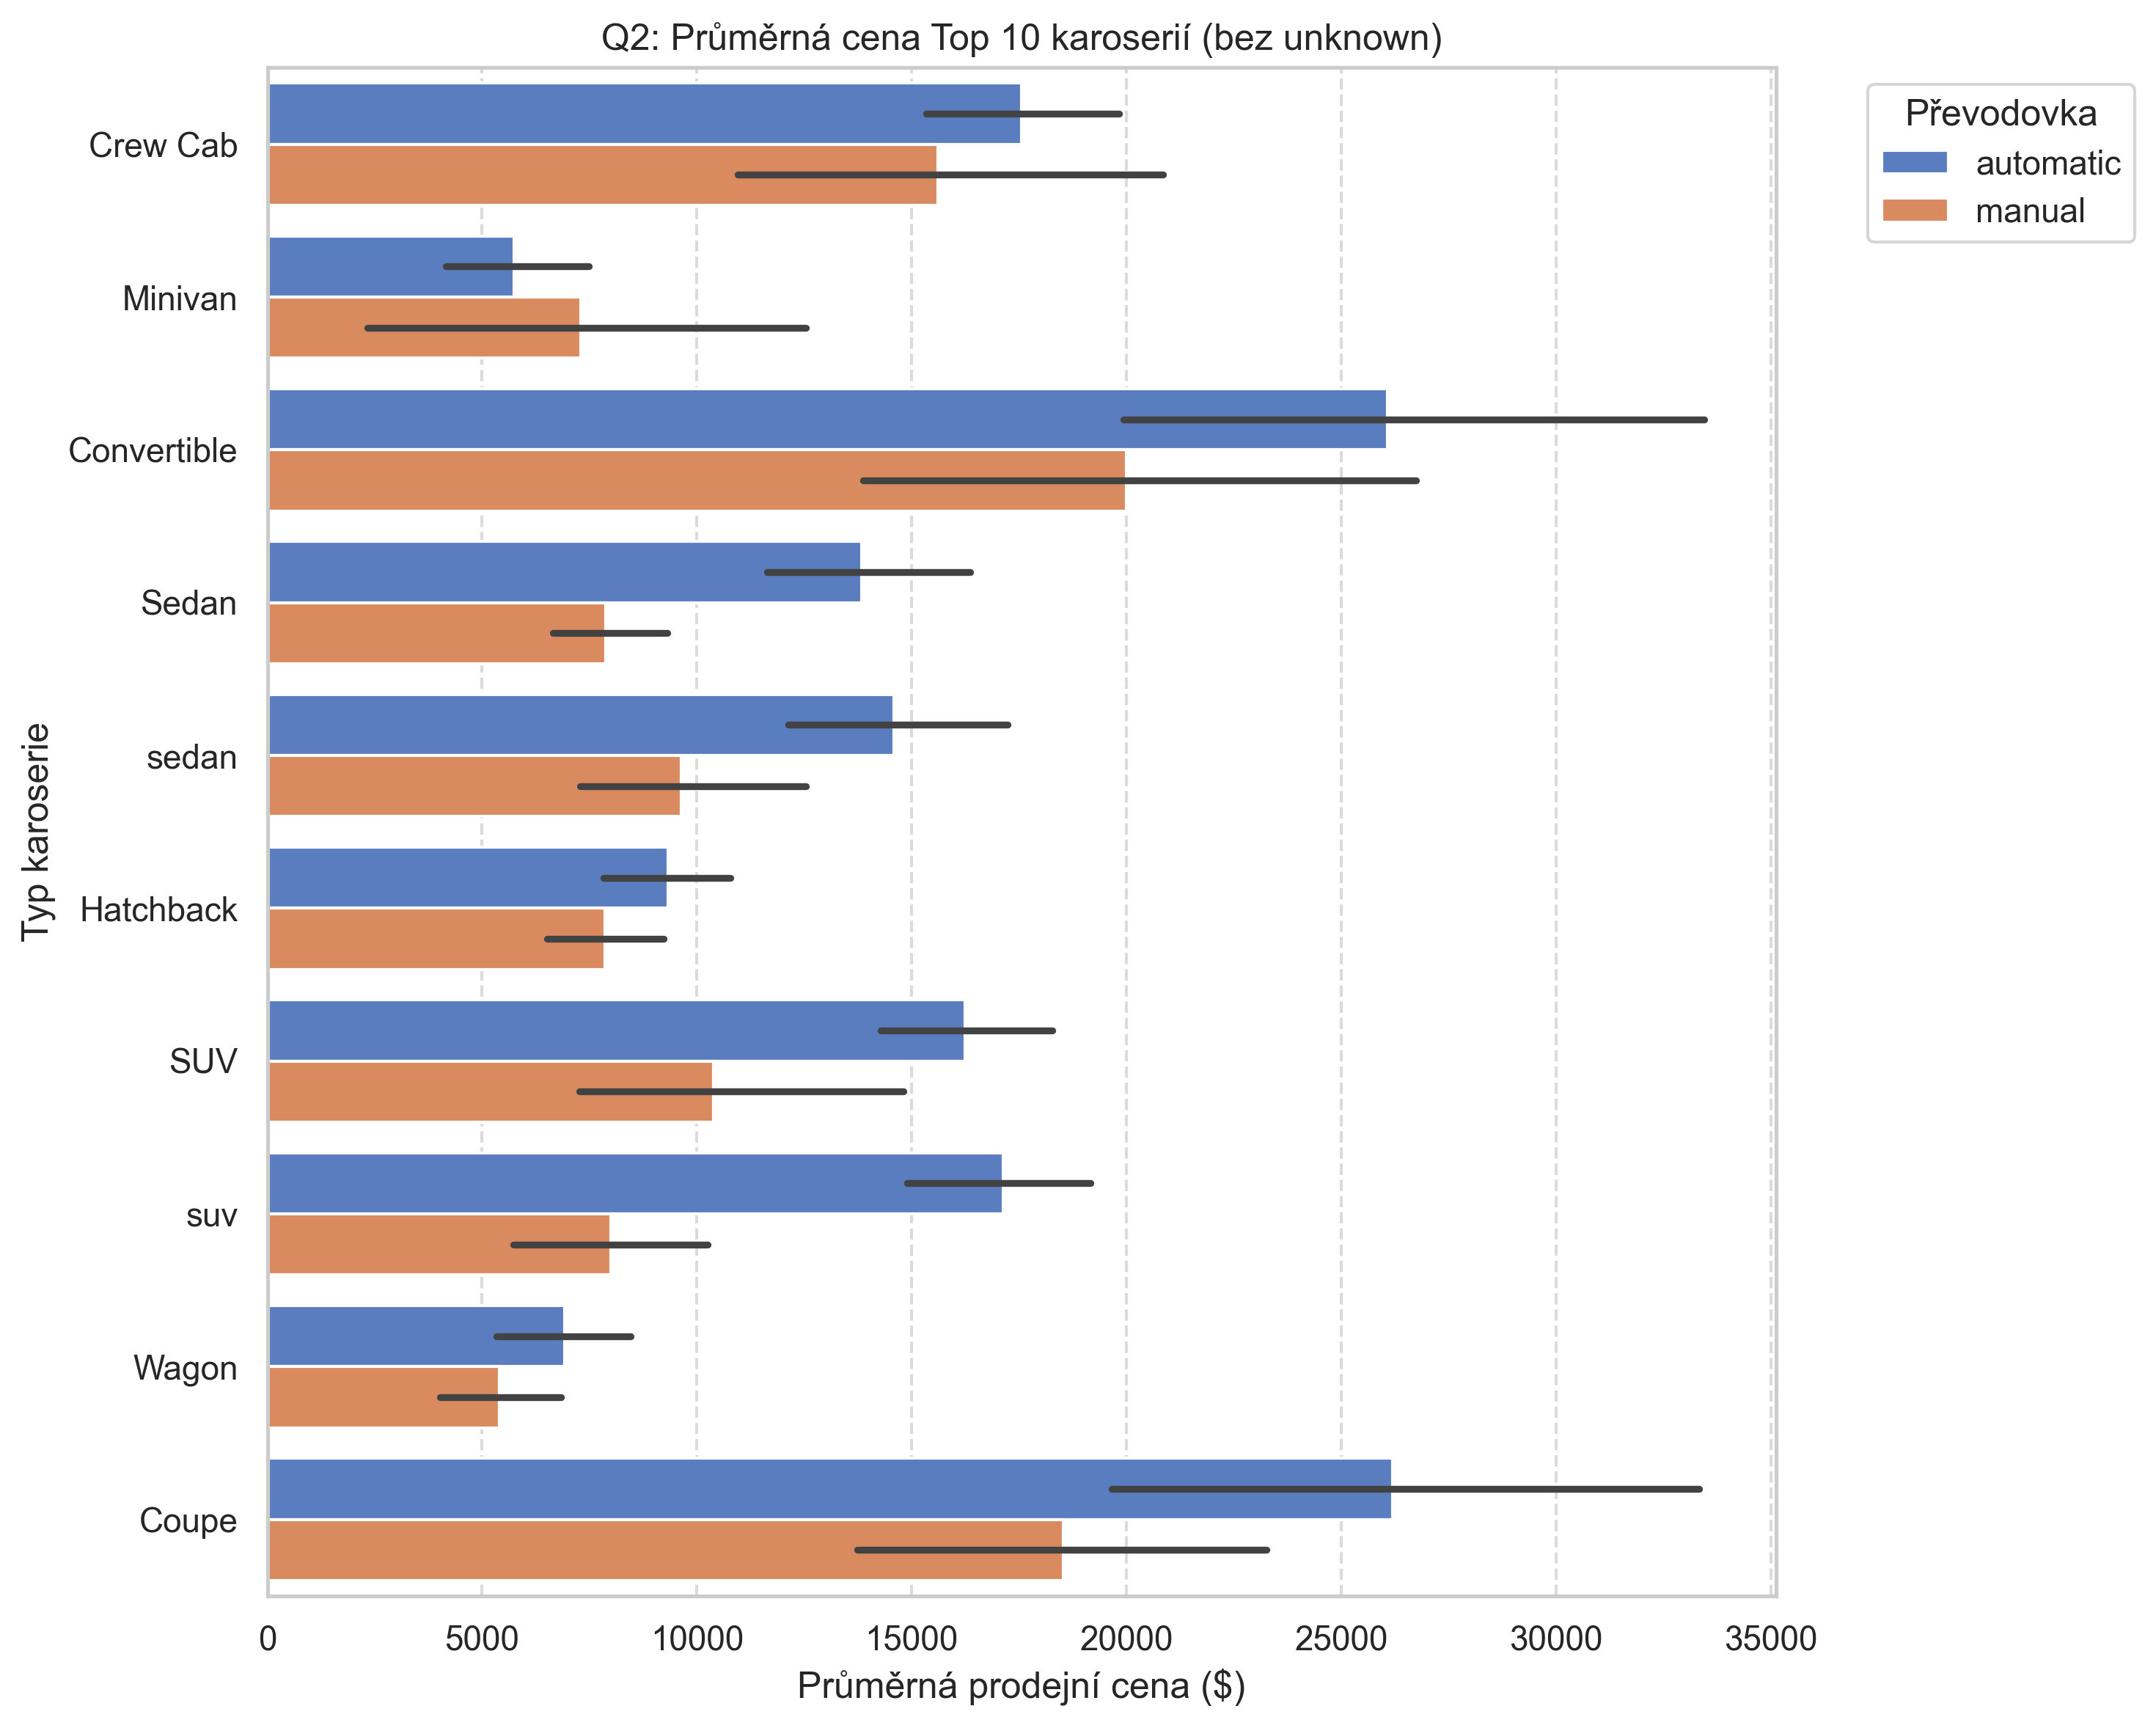
\includegraphics[width=0.9\textwidth]{../output/q2_cube_barplot.png}
    \caption{Q2 (CUBE): Horizontal bar plot top 10 karoserií – průměrná cena (\$) na x-ose, typ karoserie na y-ose, hue rozlišuje typ převodovky (Automatic/Manual). Odhaluje cenové rozdíly v kombinacích body×transmission.}
\end{figure}

% V sekci "6.4 Q3: GROUPING SETS":
   // po SQL kódu a výsledcích analýzy
\begin{figure}[H]
    \centering
    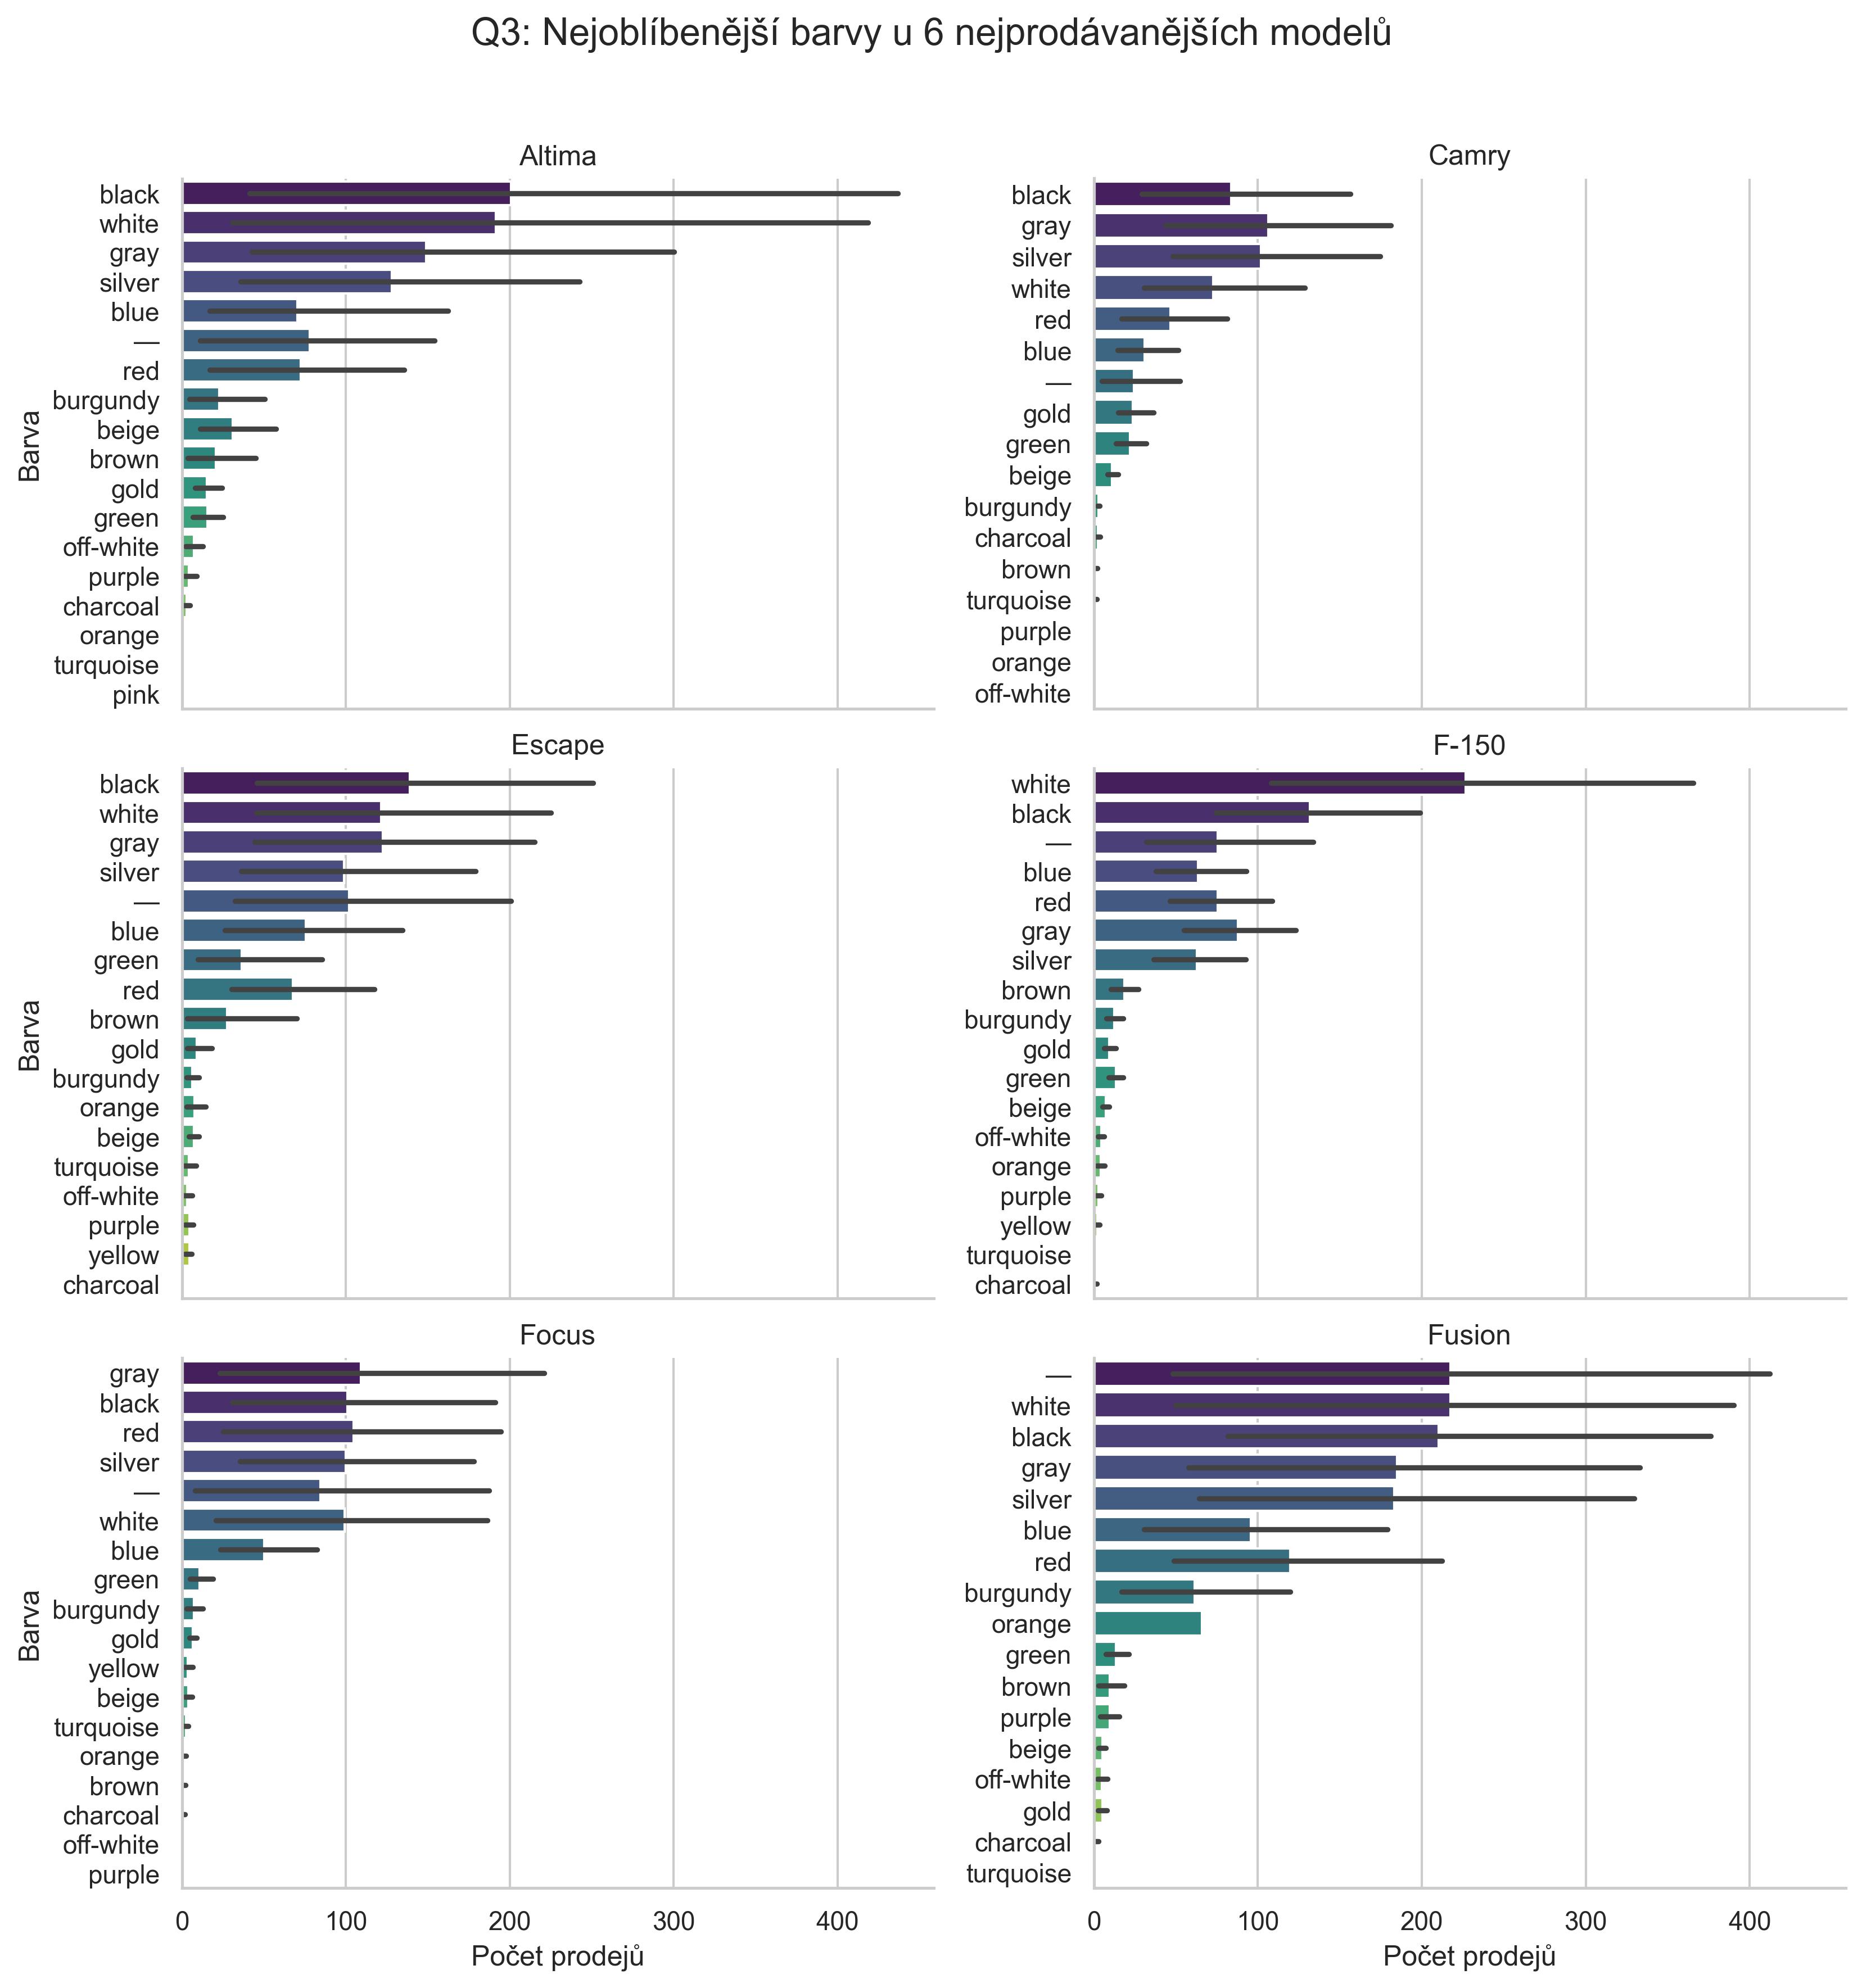
\includegraphics[width=0.85\textwidth]{../output/q3_facetgrid.png}
    \caption{Q3 (GROUPING SETS): Nejoblíbenější barvy u 6 nejprodávanějších modelů – FacetGrid vizualizace s výrazem jednotlivých barevných preferencí dle modelu}
\end{figure}

% V sekci "6.4 Q4: ROLLUP Make-Body":
   // po vysvětlení heatmapy
\begin{figure}[H]
    \centering
    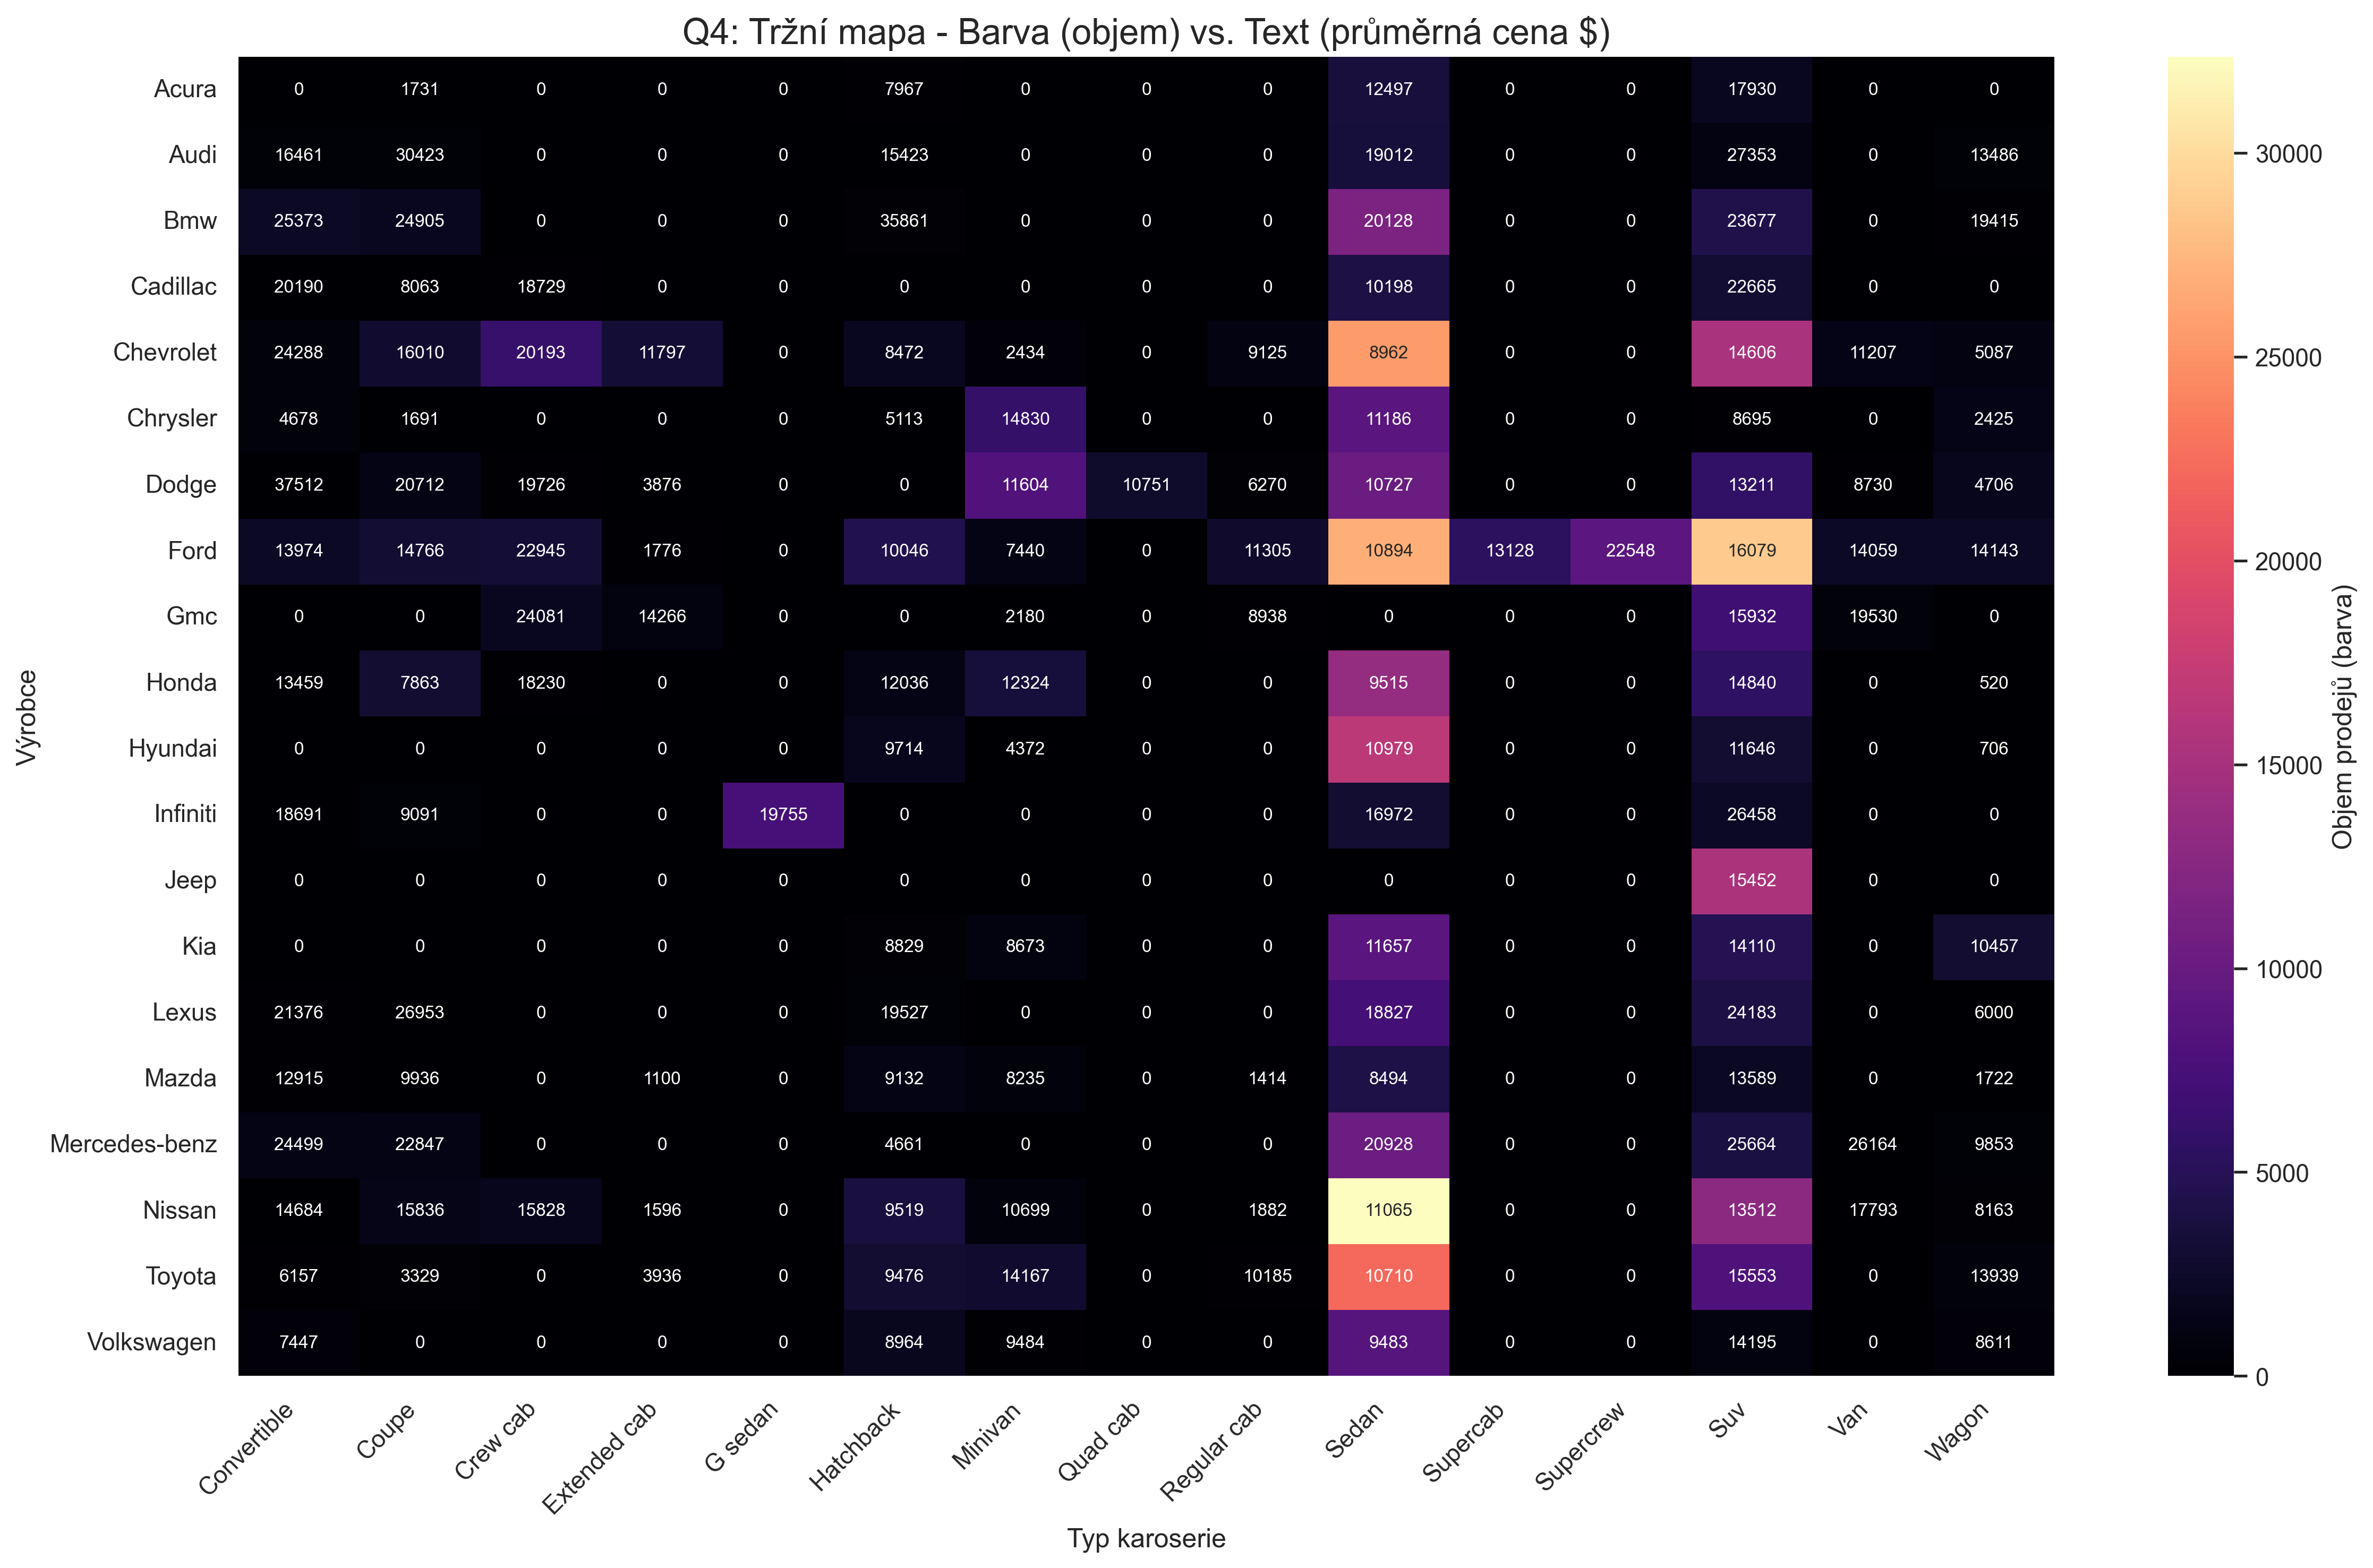
\includegraphics[width=0.9\textwidth]{../output/q4_heatmap.png}
    \caption{Q4 (ROLLUP): Dvourozměrná tržní analýza – barva (škála Magma) reprezentuje objem prodejů, čísla v buňkách průměrnou prodejní cenu USD. Identifikuje dominantní Make-Body kombinace a cenové hladiny.}
\end{figure}

% V sekci "6.5 Q5: CUBE se segmentací":
   // po vysvětlení cenových segmentů
\begin{figure}[H]
    \centering
    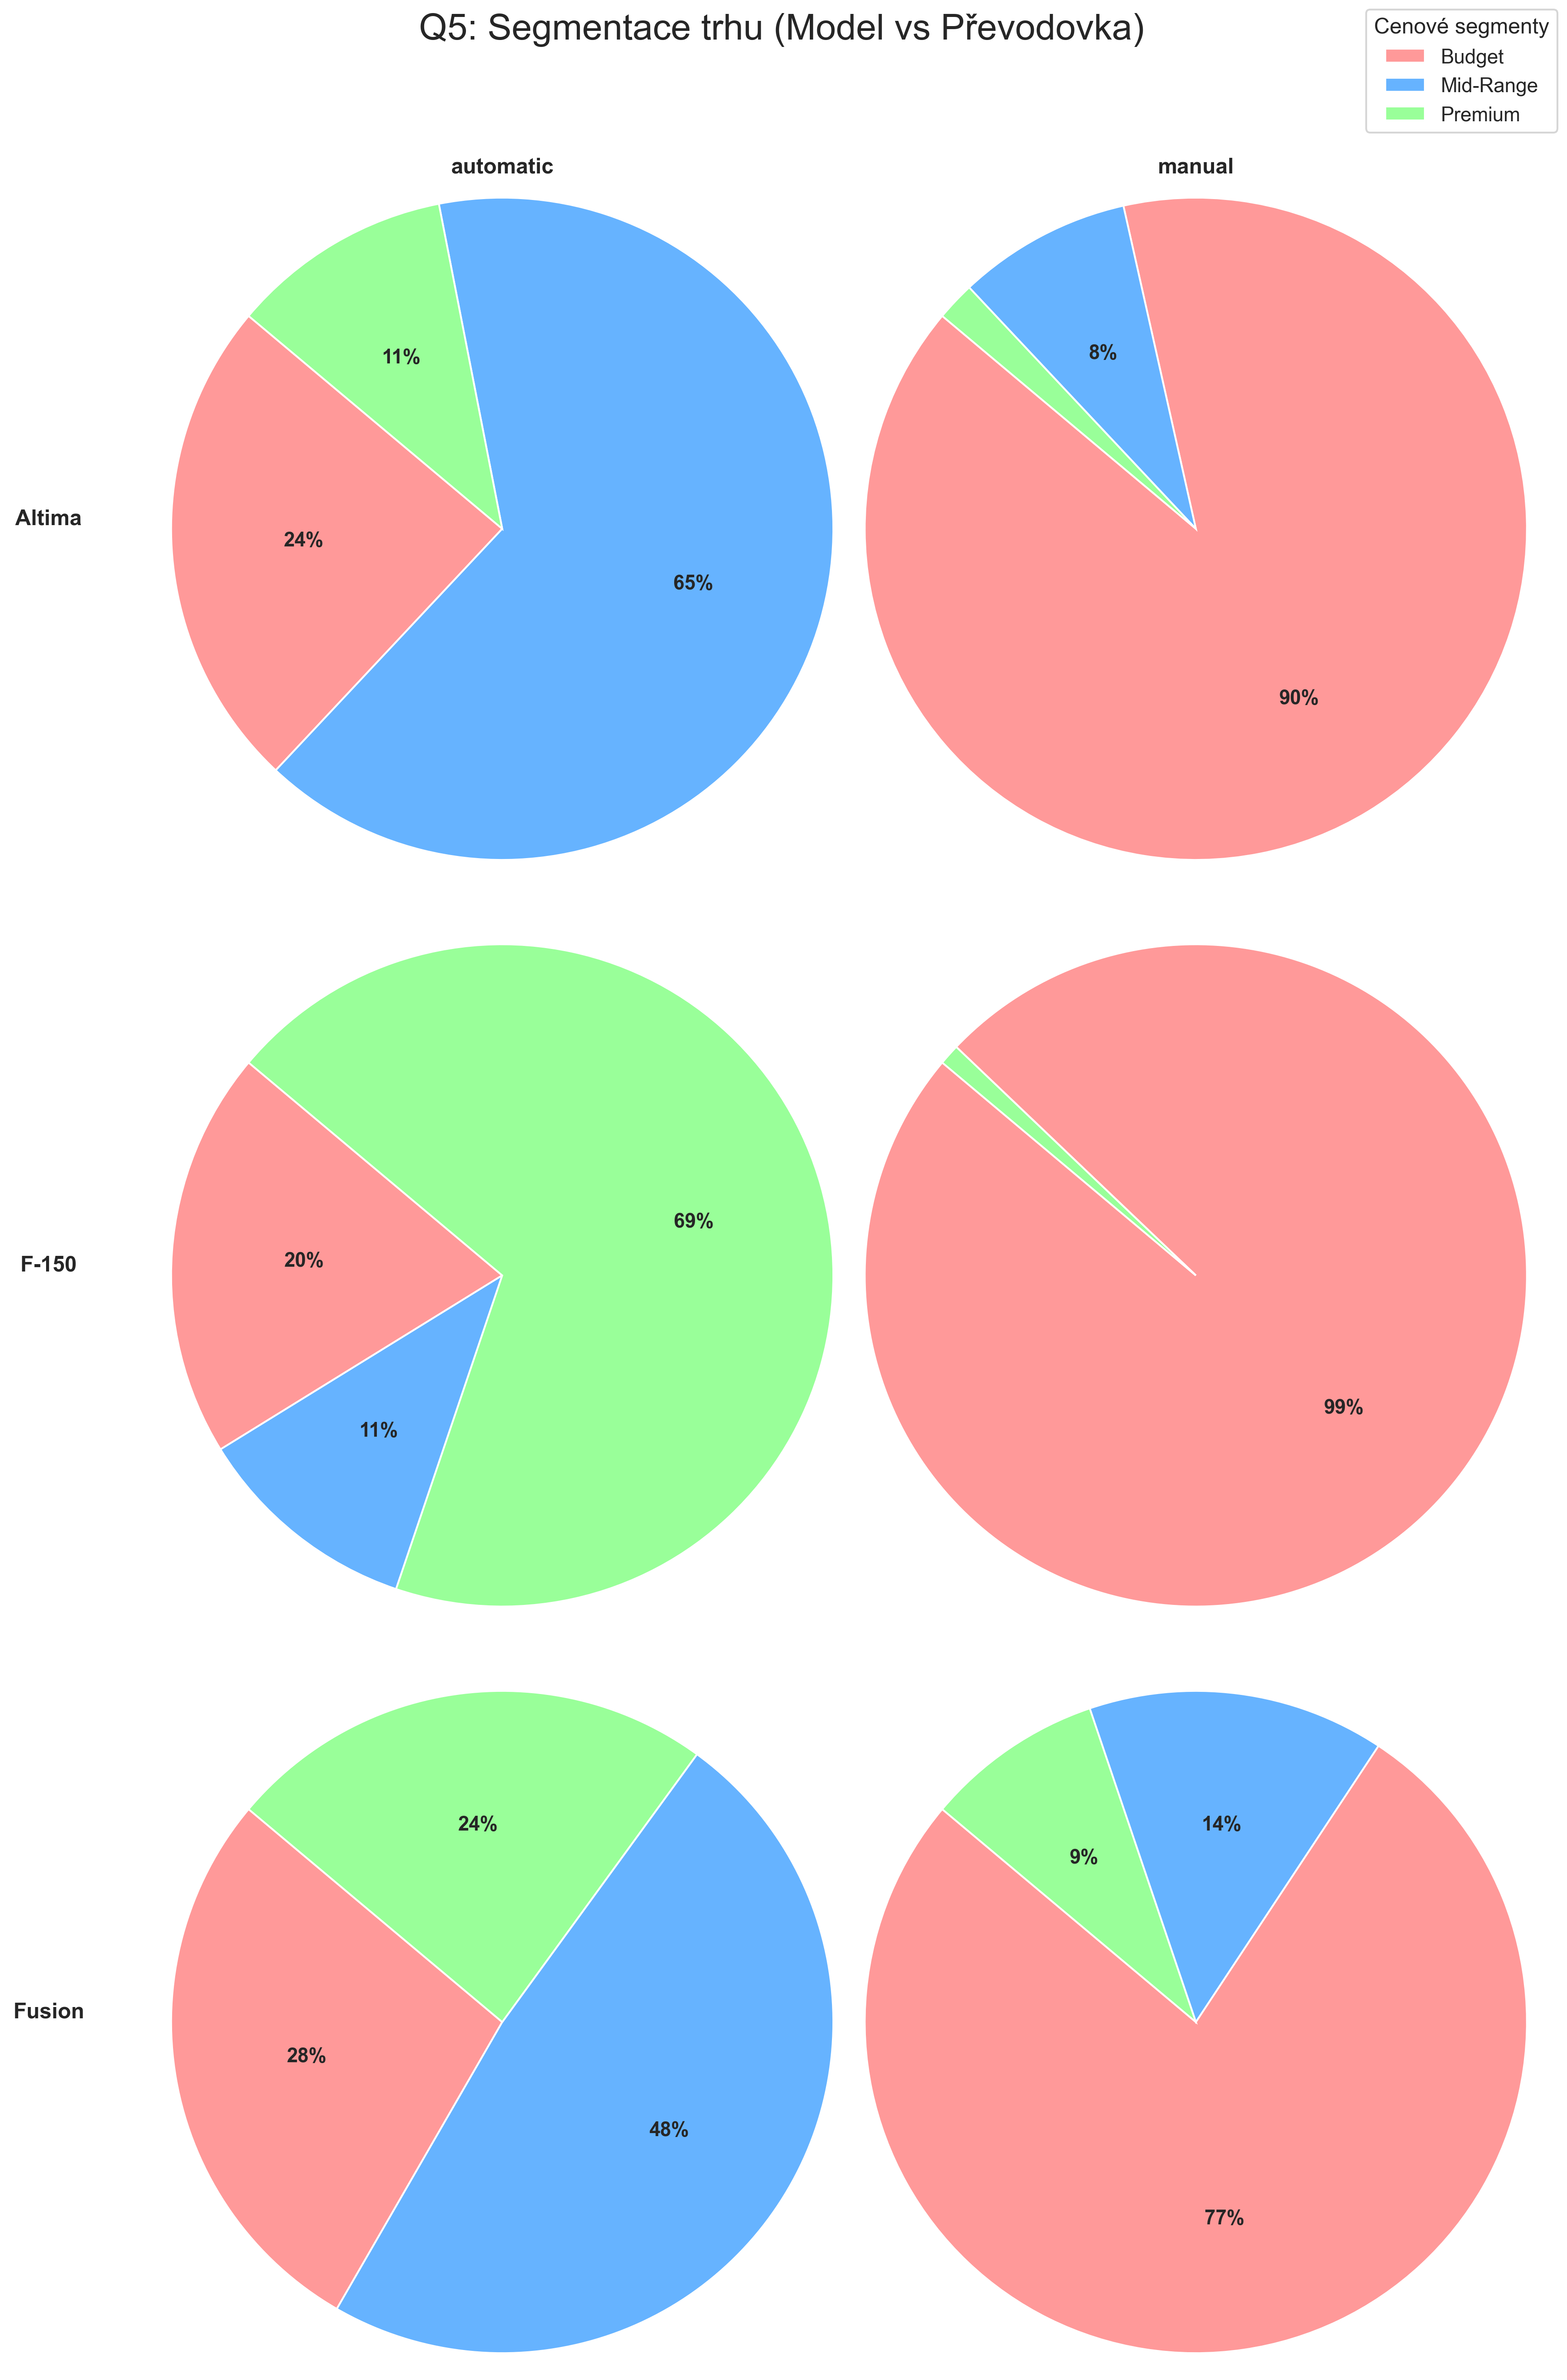
\includegraphics[width=0.95\textwidth]{../output/q5_segments_matrix.png}
    \caption{Q5 (CUBE): Segmentační matice – 3×2 grid pie chartů zobrazujících distribuci cenových segmentů (Budget/Mid-Range/Premium) pro top 3 modely dle typu převodovky (Automatic/Manual). Odhaluje "upselling" potenciál.}
\end{figure}

% V sekci "6.6 Q6: Multi-dimensional GROUPING SETS":

   % Pohled 1: Produktový - Top modely
\begin{figure}[H]
    \centering
    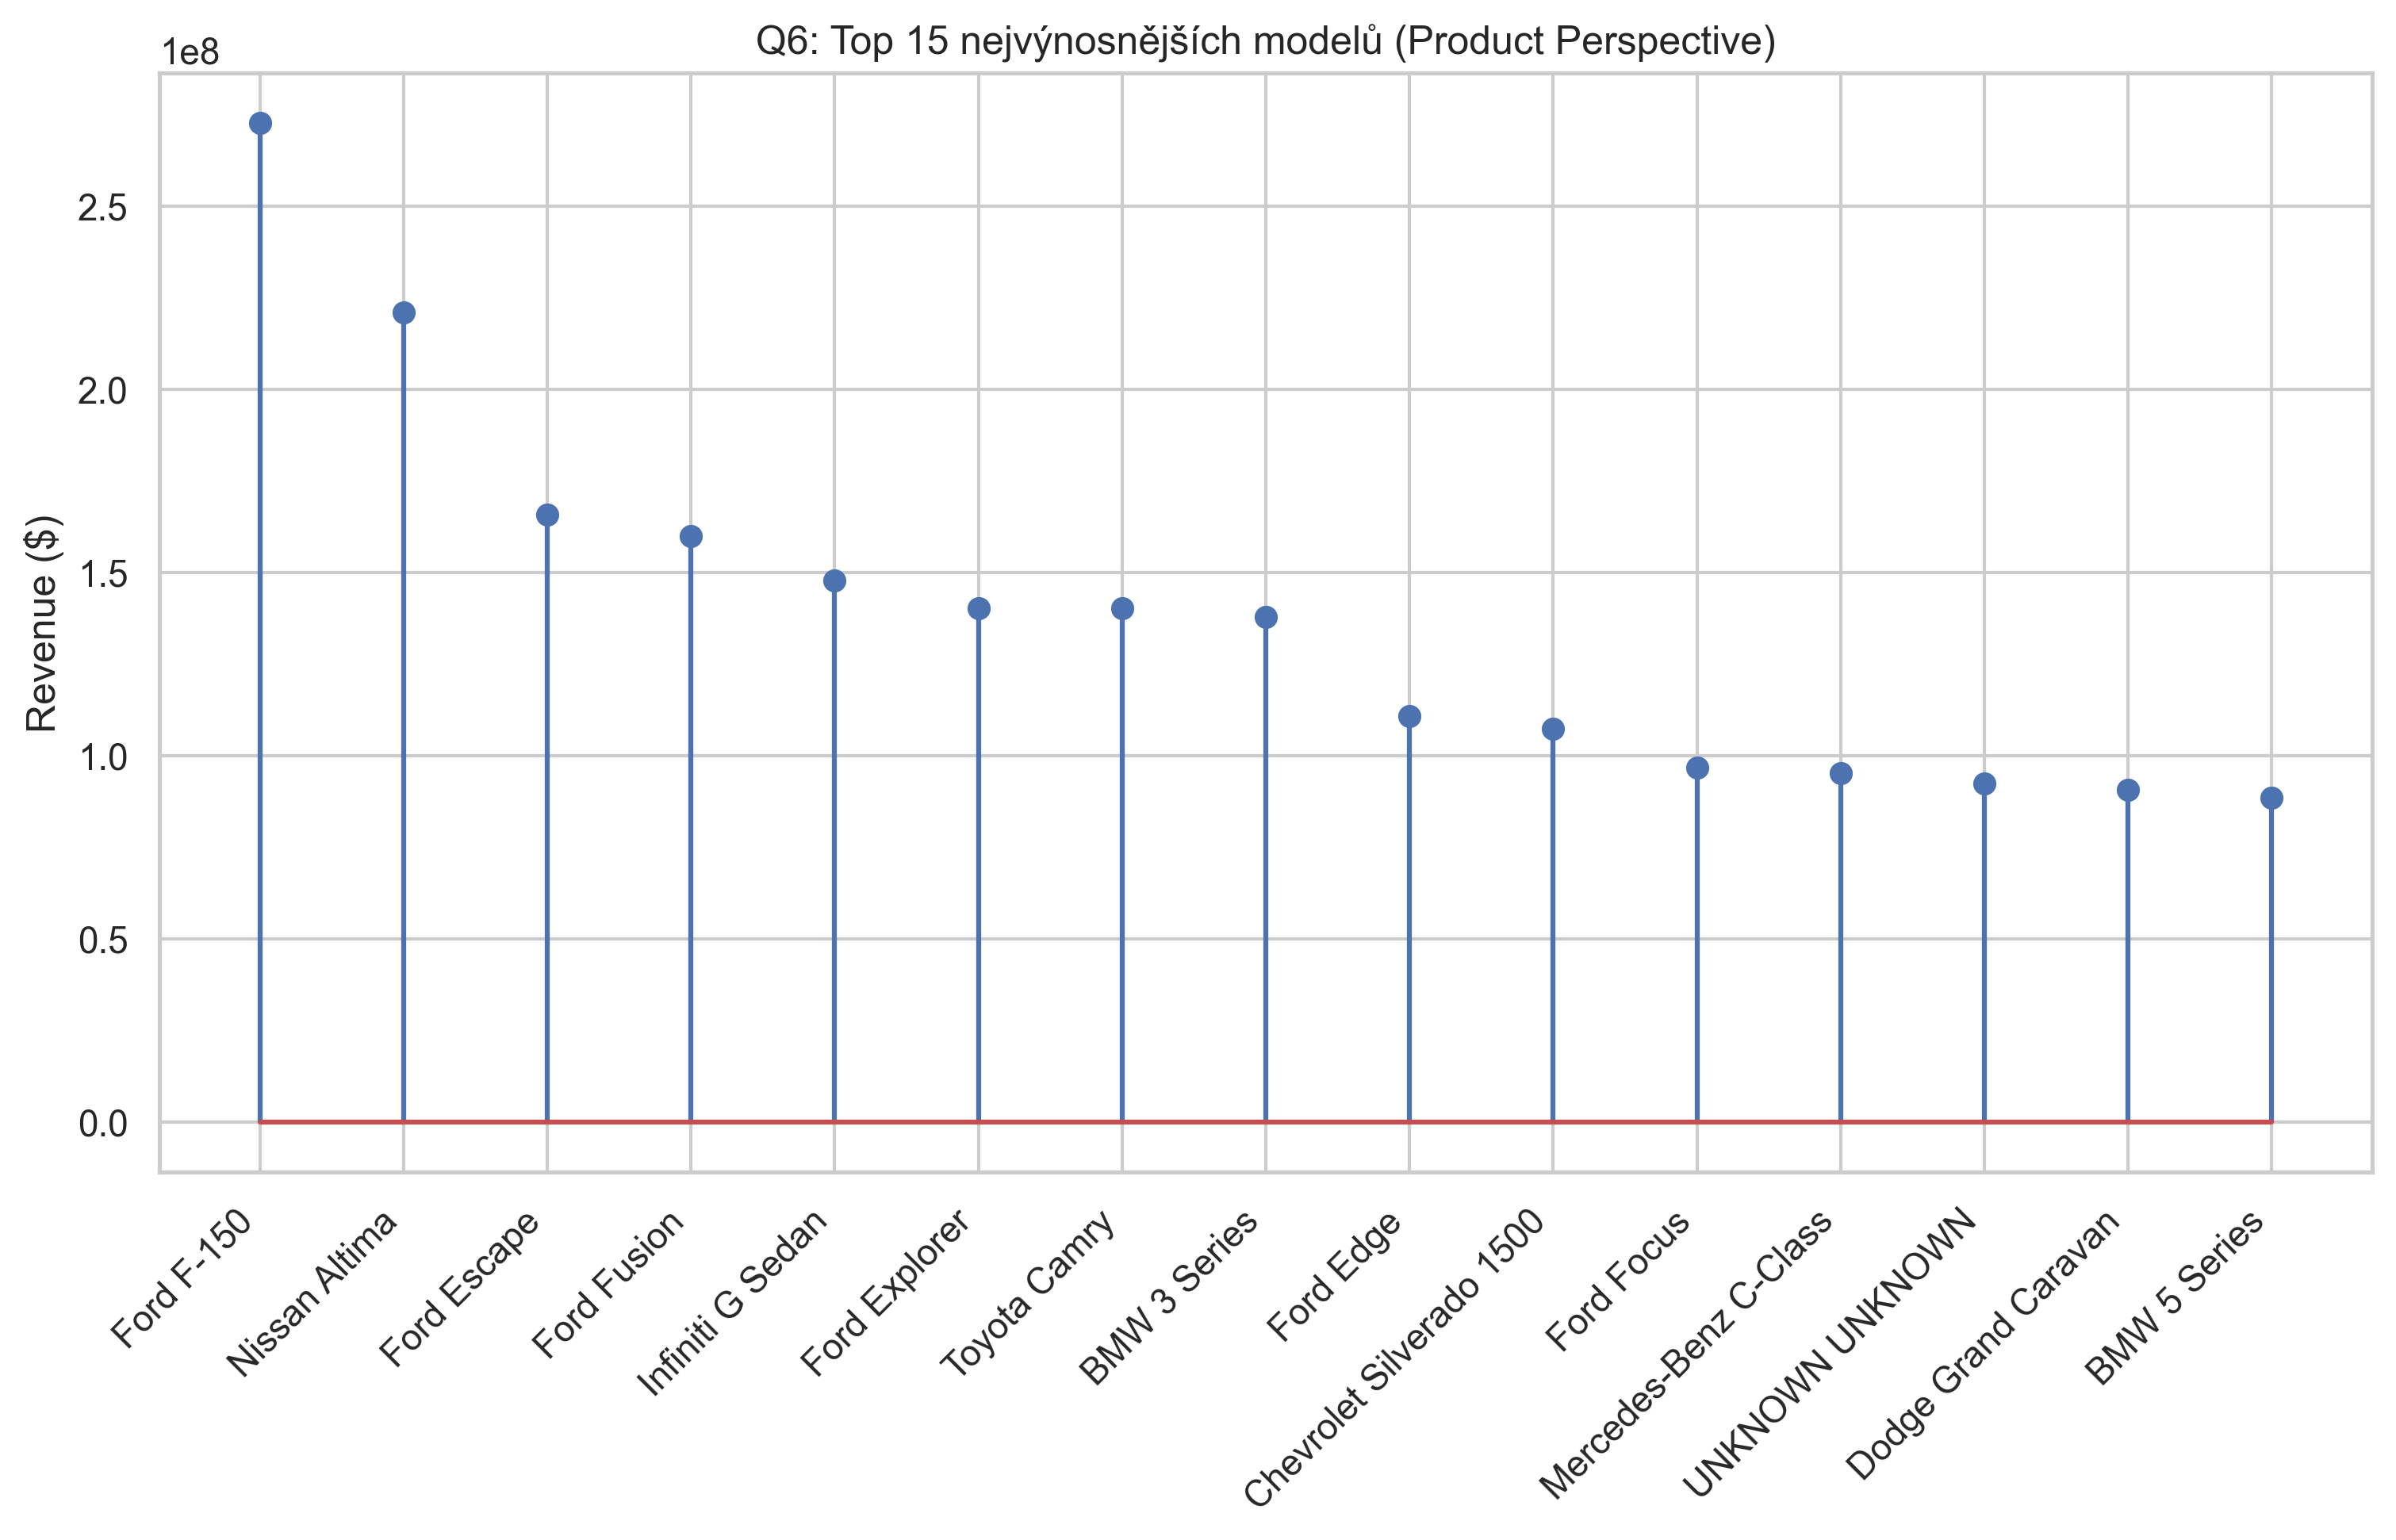
\includegraphics[width=0.85\textwidth]{../output/q6_product_analysis.png}
    \caption{Q6 (Produktový pohled): Stem plot top 15 nejvýnosnějších kombinací Značka+Model. Vizualizuje celkový výnos (total\_revenue) z jednotlivých modelů (GROUPING SETS, sada 1).}
\end{figure}

   % Pohled 2: Strukturální - Trendy karoserií v čase
\begin{figure}[H]
    \centering
    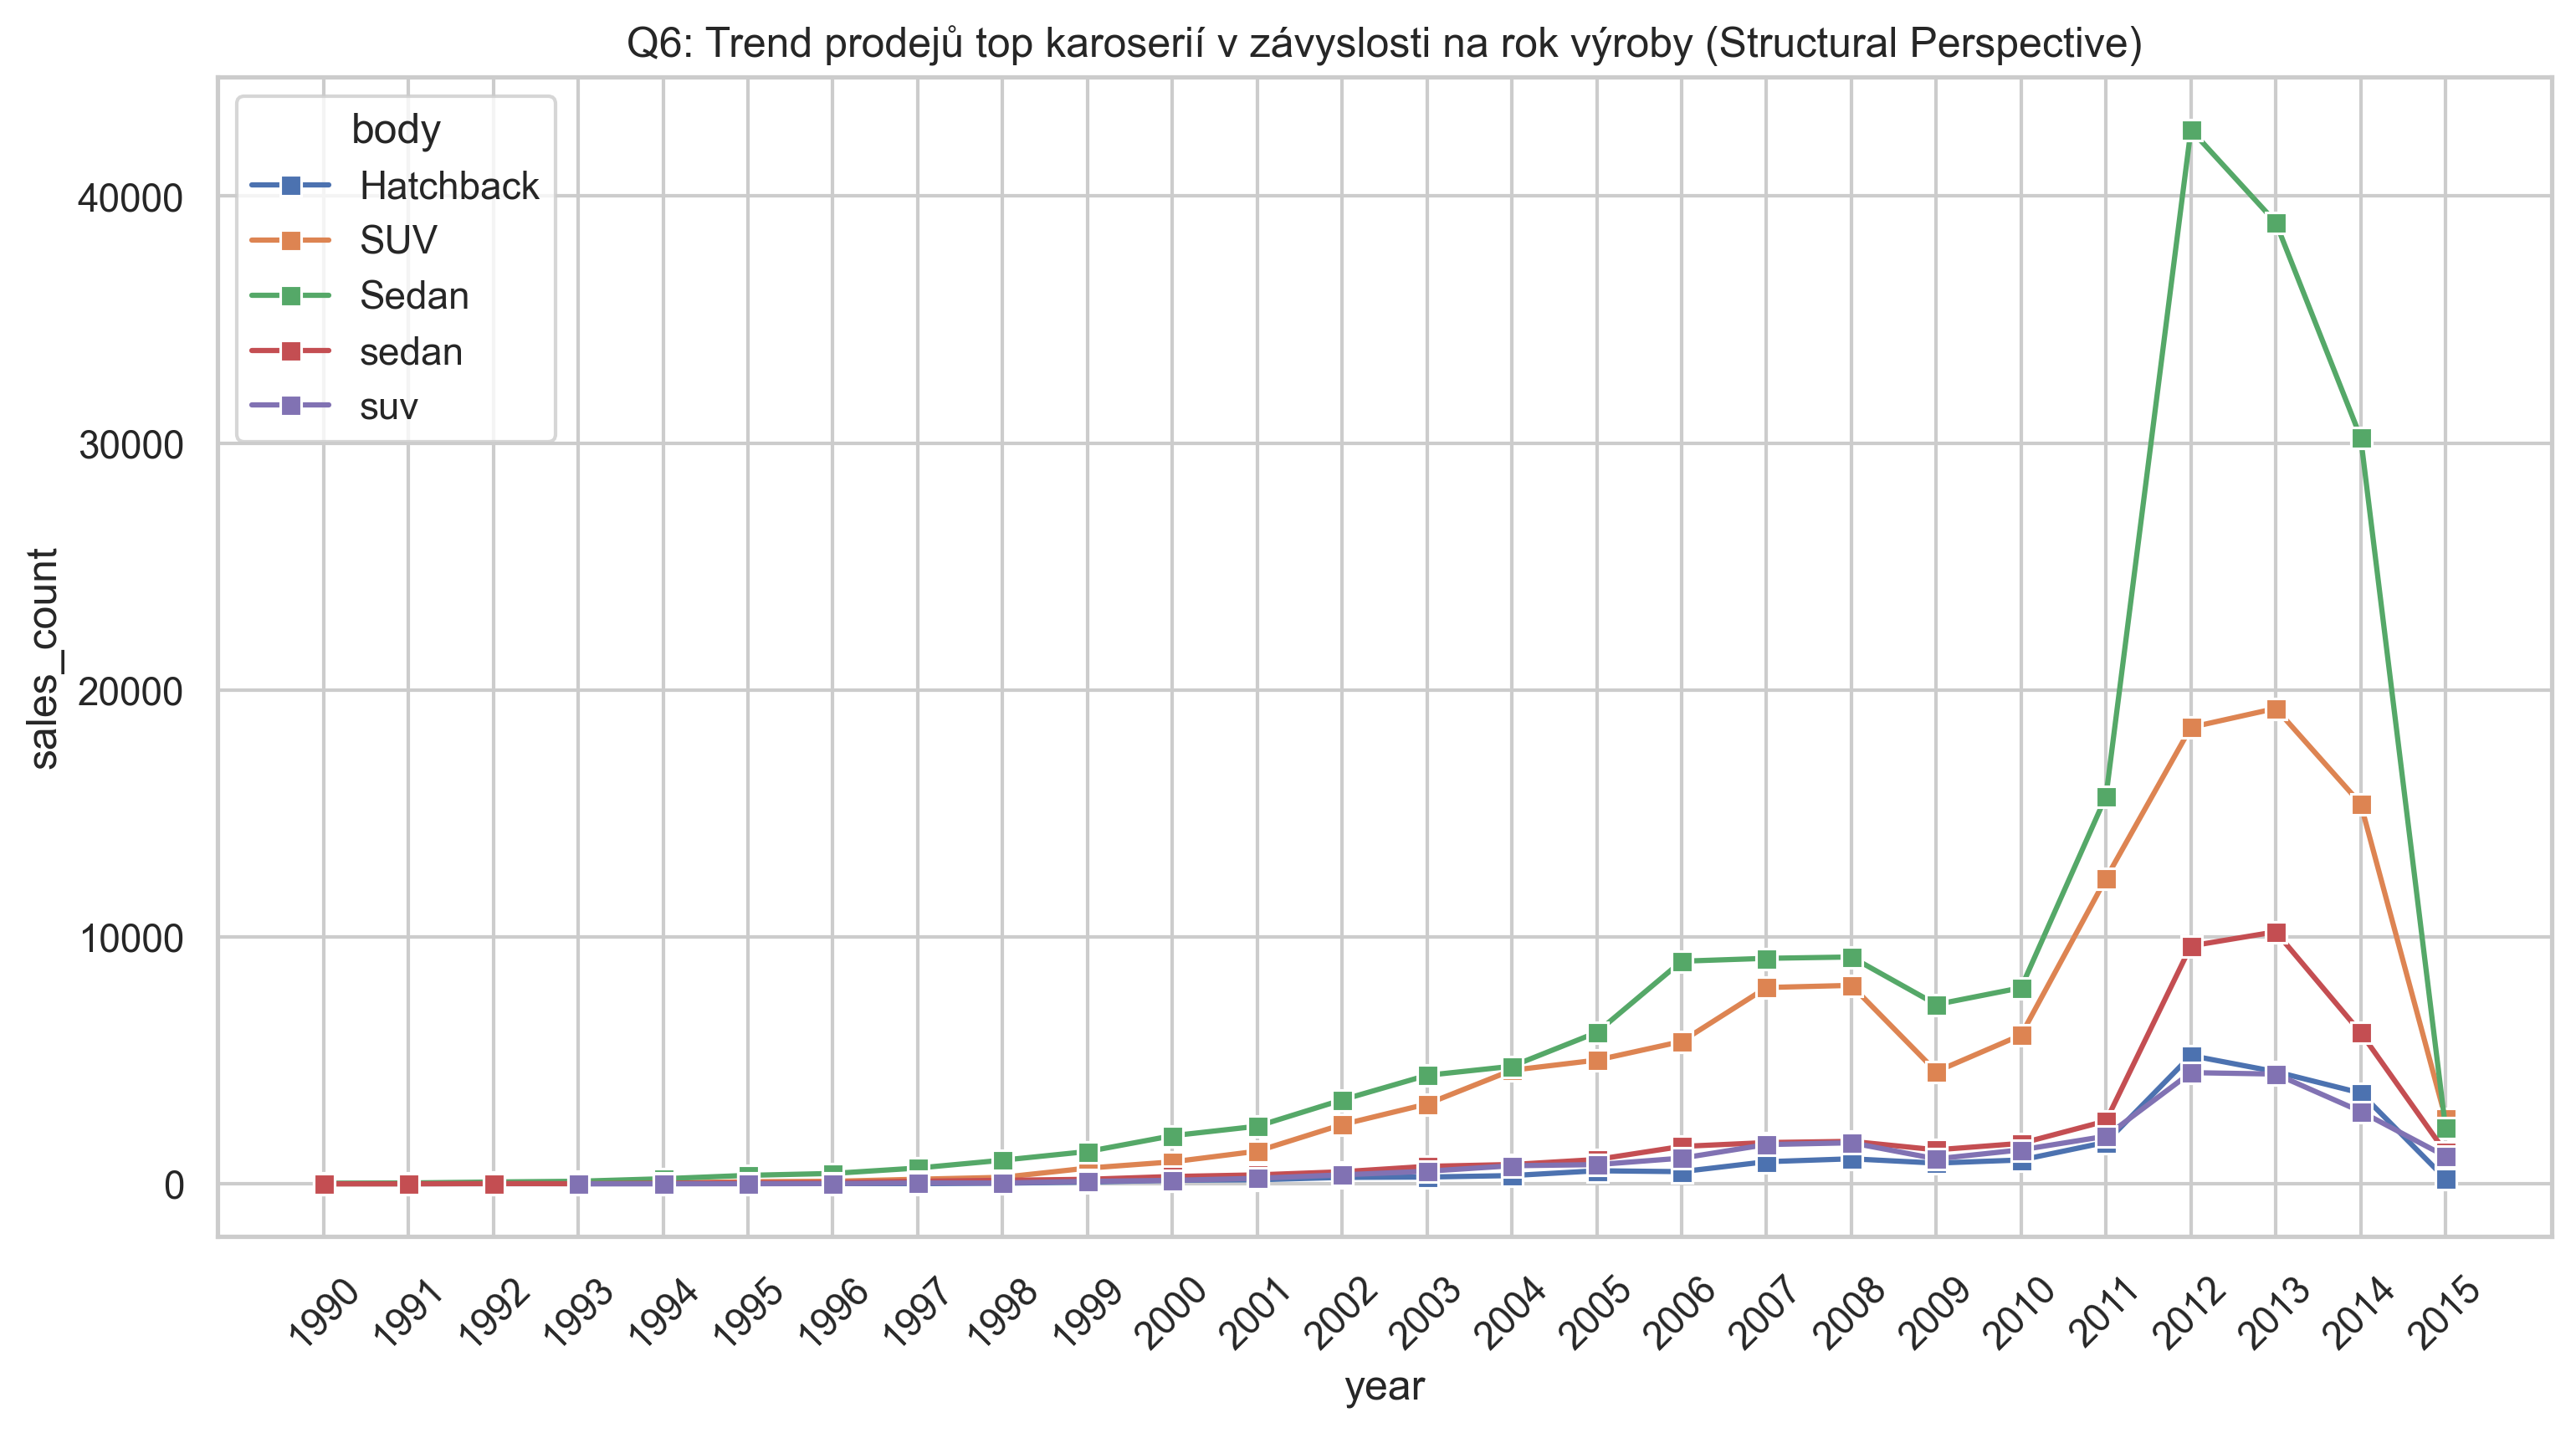
\includegraphics[width=0.85\textwidth]{../output/q6_body_trends.png}
    \caption{Q6 (Strukturální pohled): Lineplot trendů prodejů top 5 karoserií v závislosti na roce výroby. Zobrazuje časový vývoj segmentů (Sedan, SUV, Truck apod.) a jejich růst/pokles v historickém kontextu (GROUPING SETS, sada 2).}
\end{figure}

% ============================================================================
% VOLITELNÁ ROZŠÍŘENÍ (Pro Data Mining sekci)
% ============================================================================

% V sekci "8. Data Mining - A. Clustering":
   \begin{figure}[H]
       \centering
       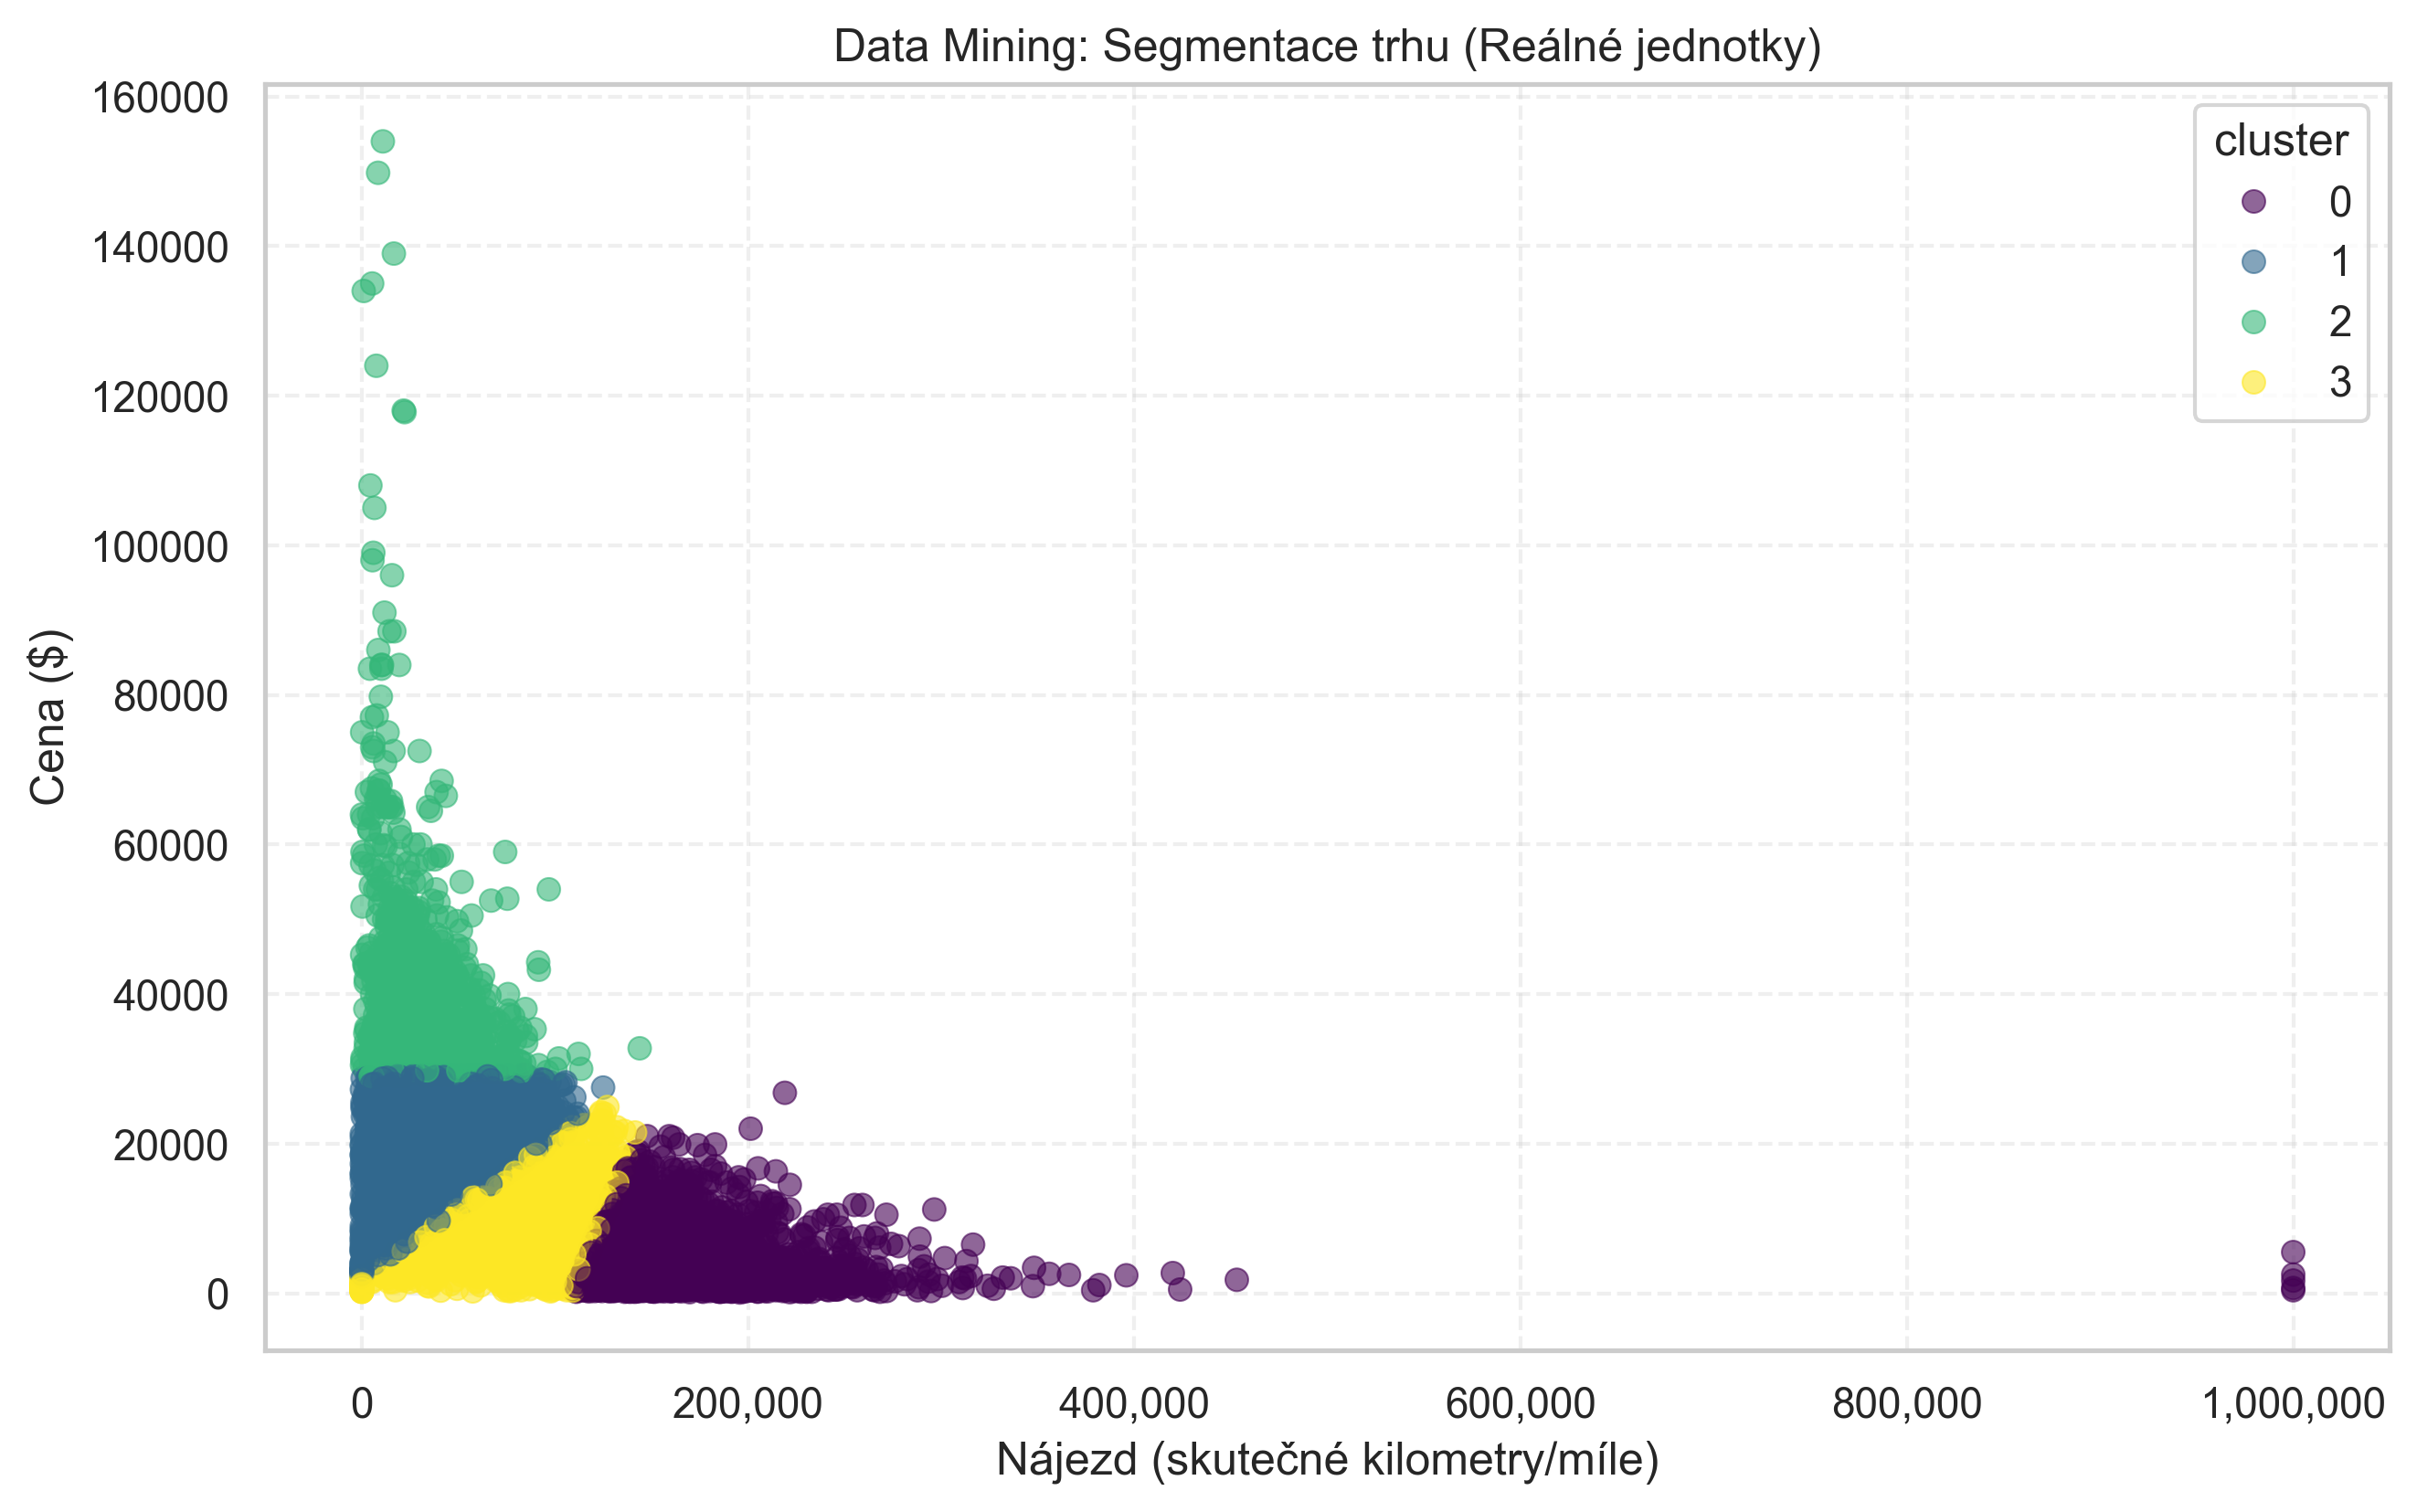
\includegraphics[width=0.85\textwidth]{../output/kmeans_scatter.png}
       \caption{K-Means segmentace (k=4): Scatter plot s reálnými jednotkami – Nájezd (km/míle) vs. Prodejní cena (\$). Barvy reprezentují 4 zjištěné shluky trhu: Prémiové kousky, Běžné vozidlo, Vozidlo na dojetí, Levné vozidlo.}
   \end{figure}

% V sekci "8. Data Mining - B. Regrese":
   \begin{figure}[H]
       \centering
       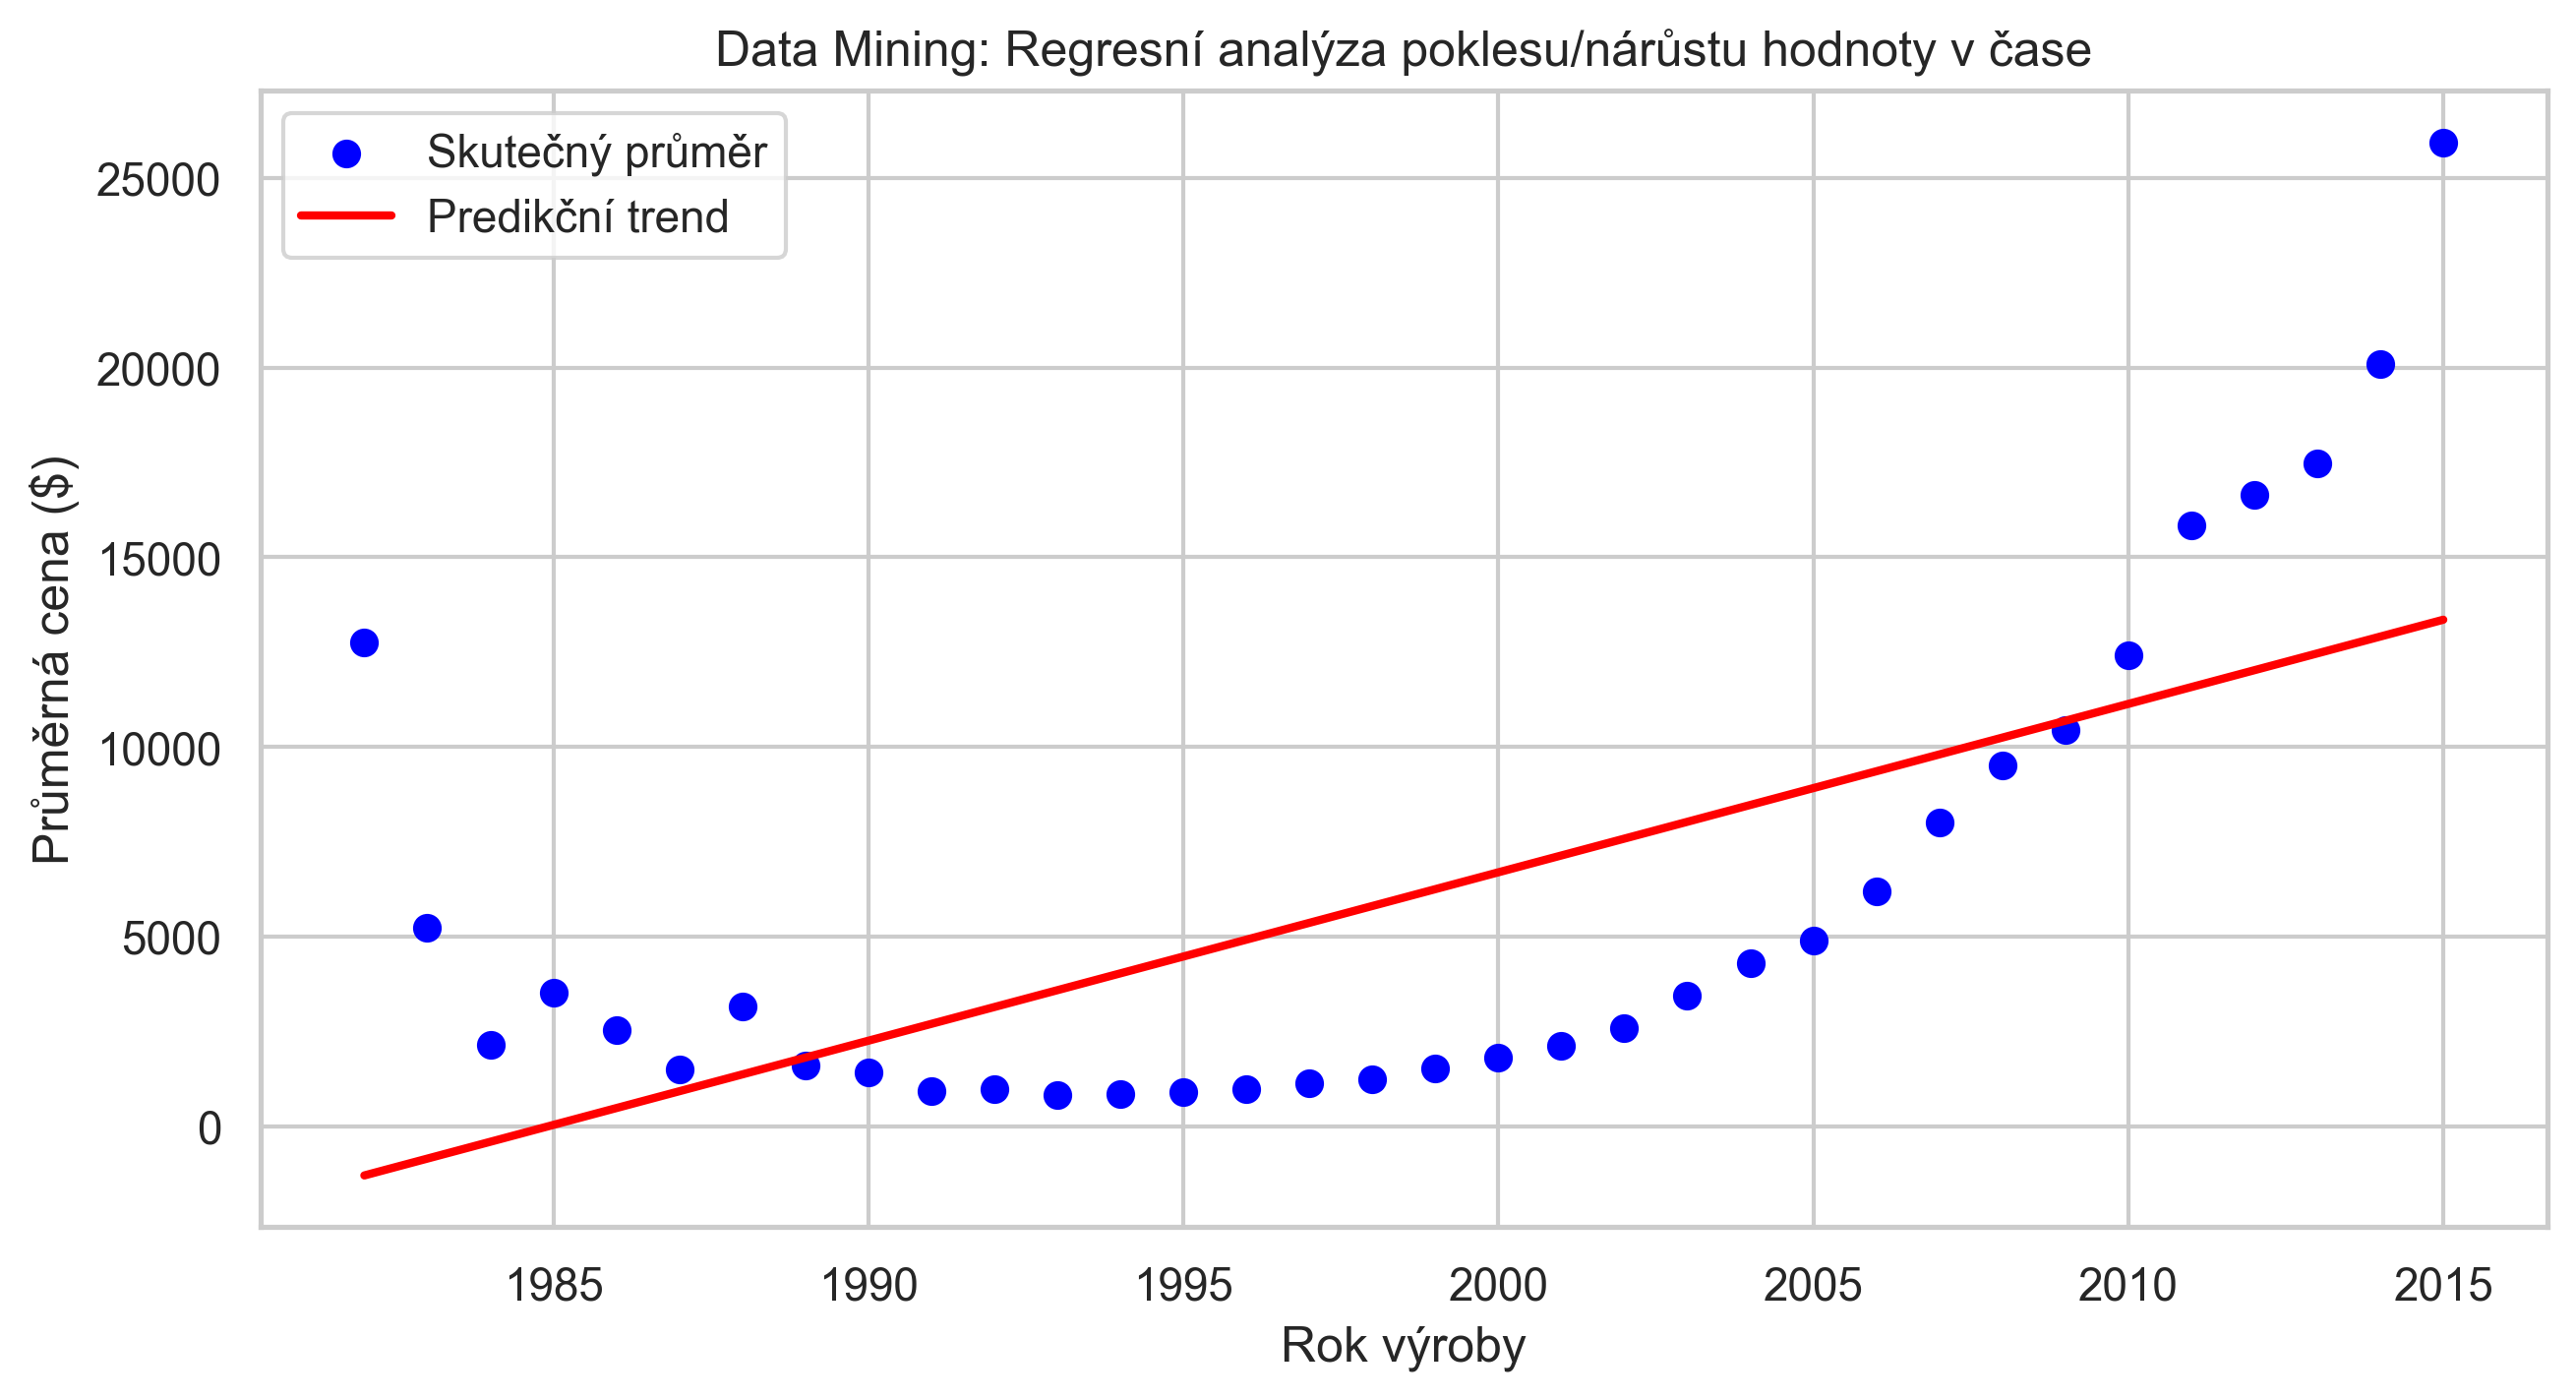
\includegraphics[width=0.85\textwidth]{../output/regression_trend.png}
       \caption{Lineární regrese: Scatterplot skupin (modré body) se schematem LOWESS/lineárního trendu (červená čára). Vyjadřuje průměrnou cenu automobilu jako funkci roku výroby – negativní sklon indikuje pokles hodnoty stářím.}
   \end{figure}

% V sekci "8. Data Mining - C. Anomálie":
   \begin{figure}[H]
       \centering
       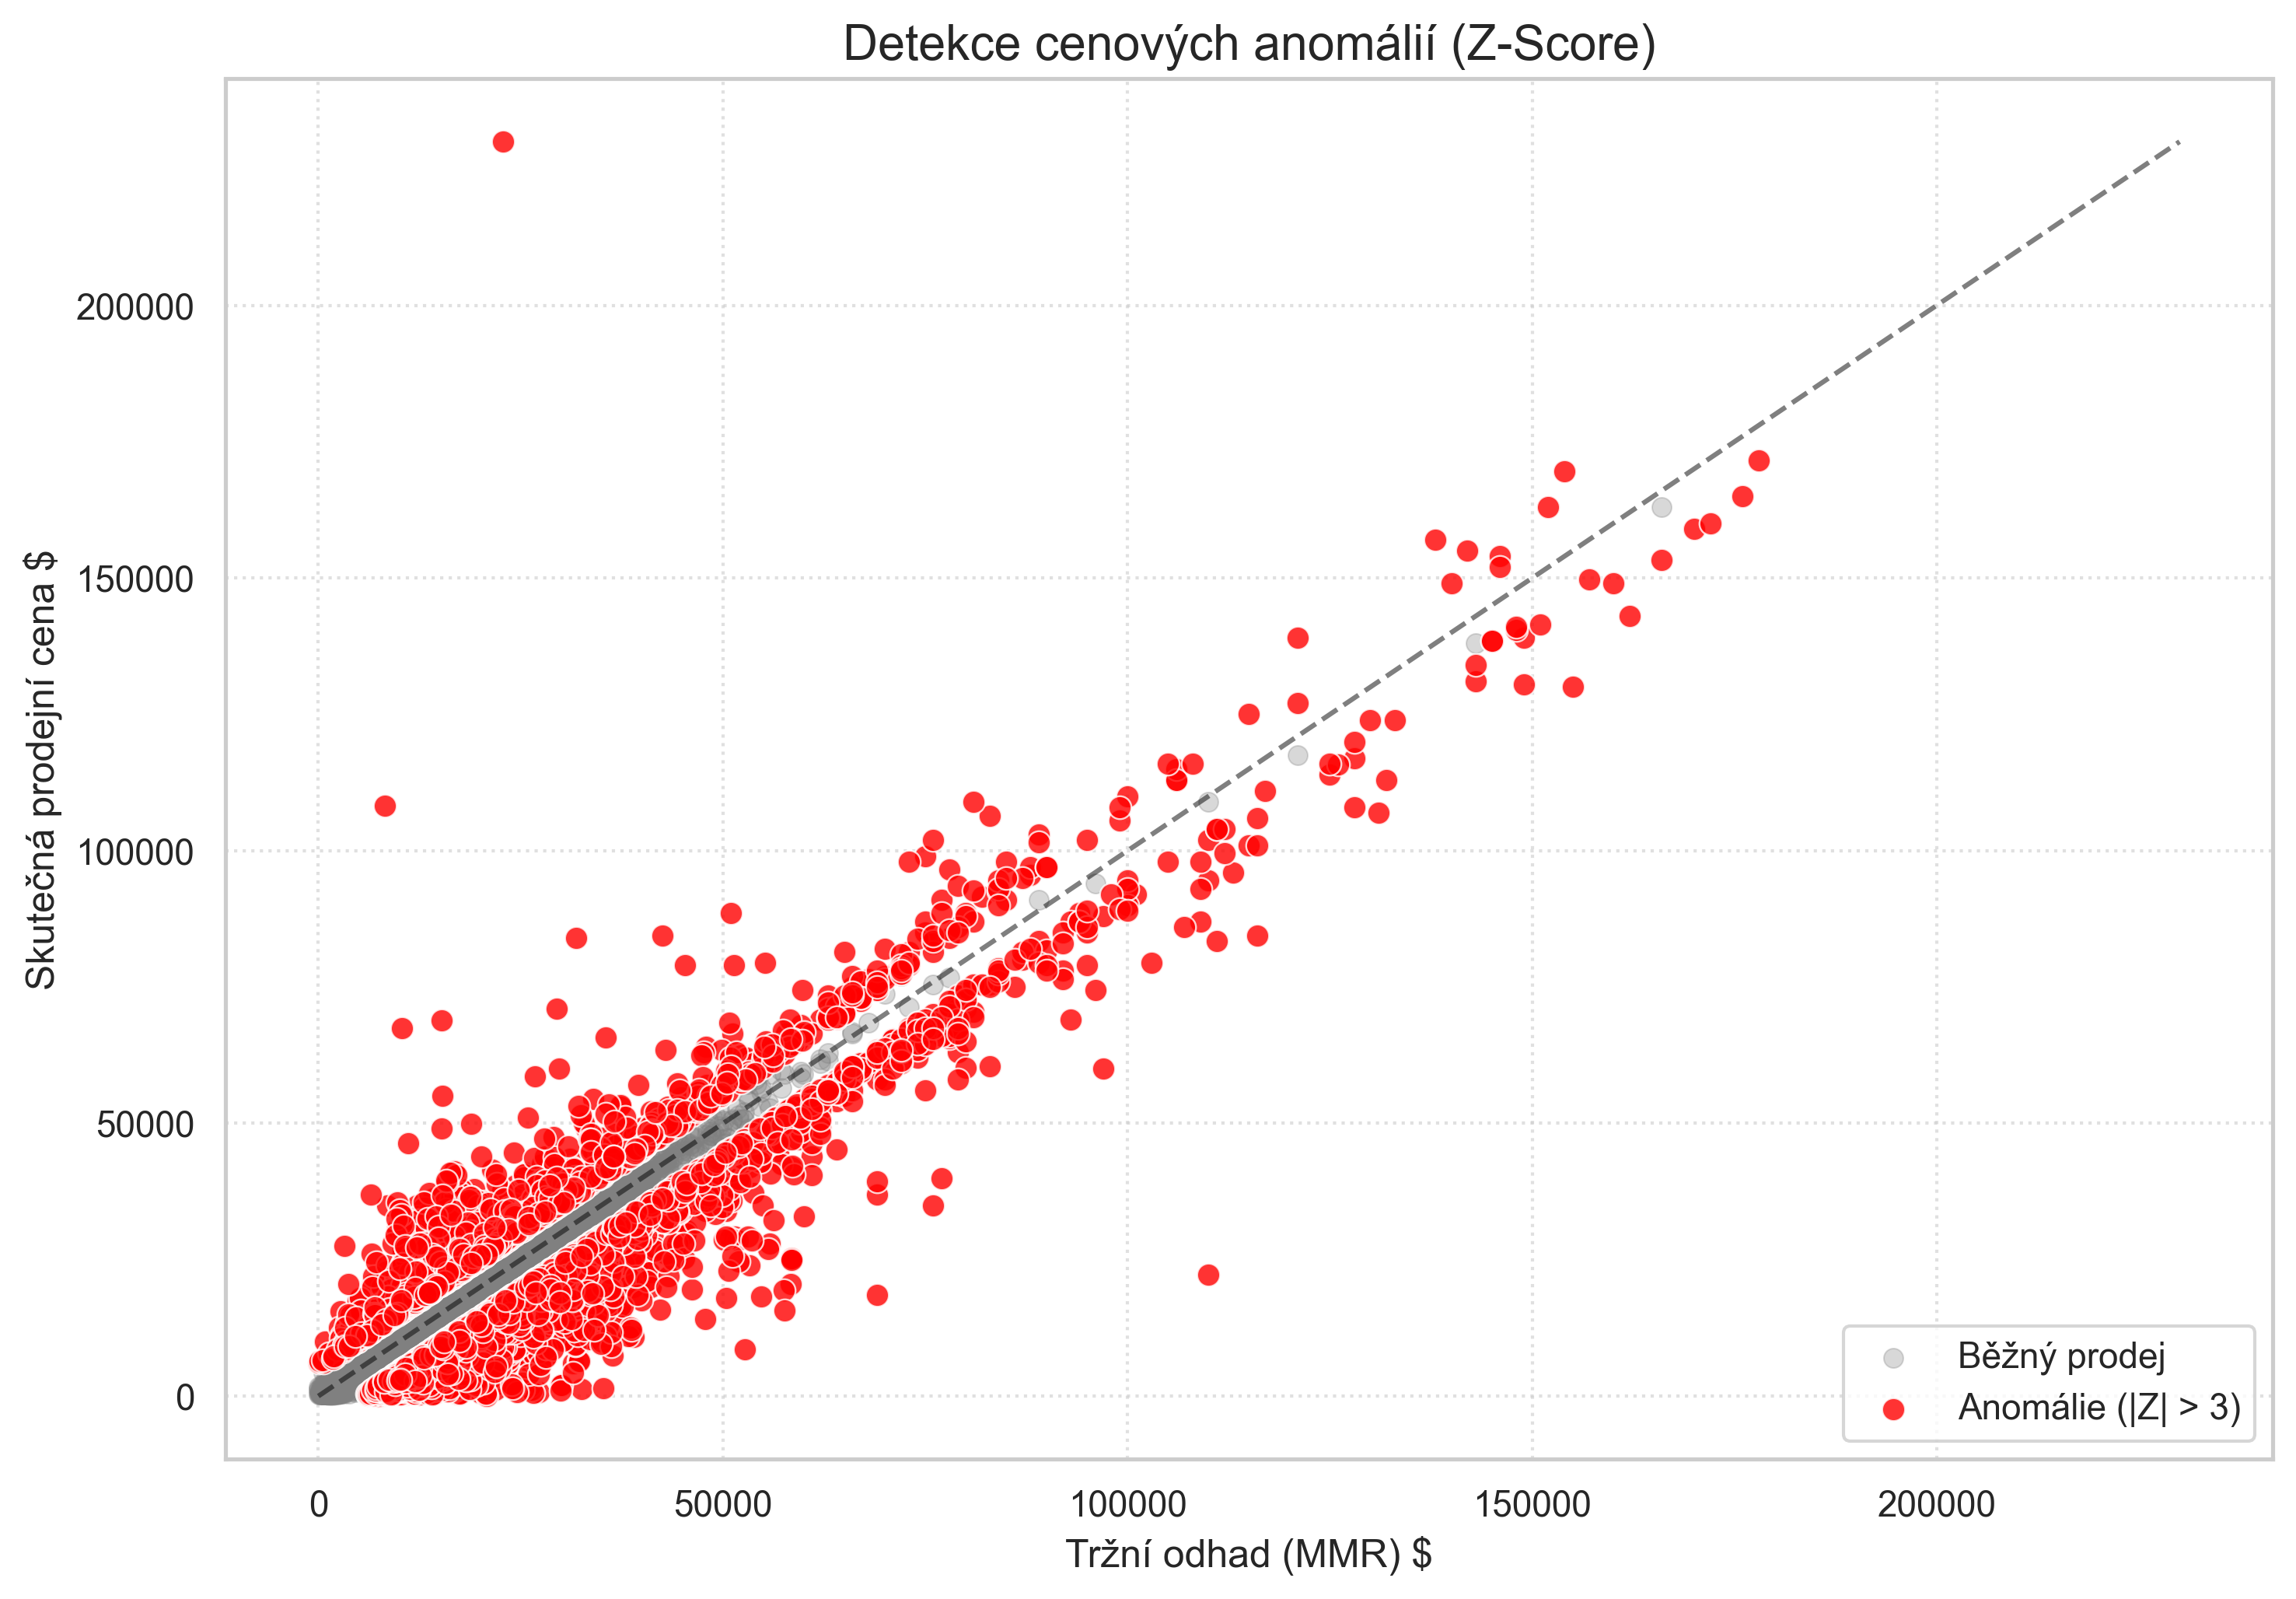
\includegraphics[width=0.85\textwidth]{../output/anomaly_detection.png}
       \caption{Detekce cenových anomálií (Z-Score): Scatterplot prodejní ceny vs. tržního odhadu (MMR). Šedé body = běžné prodeje; Červené body = anomálie ($|Z| > 3\sigma$). Diagonála = ideální shoda. Anomálie v horní oblasti = nadhodnocení, v dolní = podhodnocení.}
   \end{figure}

% ============================================================================
% BENCHMARK SEKCE
% ============================================================================

% V sekci "7. Benchmark výsledků":
   \begin{figure}[H]
       \centering
       \includegraphics[width=0.9\textwidth]{../output/benchmark_comparison.png}
       \caption{Srovnění výkonnosti: DuckDB vs PostgreSQL na 6 OLAP queries}
   \end{figure}
